%Template pembuatan Tesis dengan ugmtesis.

\documentclass[tesis]{ugmtesis}
\usepackage{listings}
\usepackage{color}
\usepackage{tabularx}
\usepackage{pdflscape}
\DeclareGraphicsExtensions{.png}
\graphicspath{{./Img/}}
%-----------------------------------------------------------------
%Disini awal masukan untuk data tesis
%-----------------------------------------------------------------
\titleind{SISTEM \textit{QUESTION ANSWERING} DATA KABUPATEN DI NUSA TENGGARA BARAT BERBASIS MULTI-ONTOLOGI}

\titleeng{QUESTION ANSWERING SYSTEM OF COUNTY DATA IN WEST NUSA TENGGARA USING MULTI-ONTOLOGY BASED}

\fullname{SYAMSUL MUTTAQIN}

\idnum{11/323286/PPA/03632}

\examdate{}

\degree{Master of Computer Science}

\yearsubmit{2013}

\program{Ilmu Komputer}

\headprogram{Prof. Dra. Sri Hartati, Ph.D}

\dept{Ilmu Komputer}

\firstsupervisor{DR techn. Khabib Mustofa}

\firstexaminer{}

\secondexaminer{}

\thirdexaminer{}

%-----------------------------------------------------------------
%Disini akhir masukan untuk data tesis
%-----------------------------------------------------------------

\begin{document}
% ------------------------------------------------------------------------
% setting untuk listing coding OWL
% ------------------------------------------------------------------------
\lstset{language=XML, breaklines=true, keepspaces=true, columns=flexible}
% ------------------------------------------------------------------------

\cover

\titlepageind 

\approvalpage

\declarepage

%-----------------------------------------------------------------
%Disini awal masukan Acknowledment
%-----------------------------------------------------------------
\acknowledment
\begin{flushright}
\Large\emph\cal{Karya sederhana ini kupersembahkan \\
buat Bapak, Ibu, \\dan Adik-adikku tercinta}
\end{flushright}
%-----------------------------------------------------------------
%Disini akhir masukan untuk muka tesis
%-----------------------------------------------------------------

%-----------------------------------------------------------------
%Disini awal masukan Motto
%-----------------------------------------------------------------
\motto
\emph{Sesungguhnya dalam penciptaan langit dan bumi, dan silih bergantinya
malam dan siang terdapat tanda-tanda bagi orang-orang yang berakal, (yaitu)
orang-orang yang mengingat Allah sambil berdiri atau duduk atau dalam keadaan
berbaring dan mereka memikirkan tentang penciptaan langit dan bumi (seraya
berkata) : Ya Tuhan kami, tiadalah Engkau menciptakan ini dengan sia-sia, Maha
Suci Engkau, maka peliharalah kami dari siksa neraka.}

\begin{flushright}
(Q.S. Ali Imran : 190 - 191)
\end{flushright}

\emph{Maka apabila kamu telah selesai (dari sesuatu urusan), kerjakanlah
dengan sungguh-sungguh (urusan) yang lain.}

\begin{flushright}
(Q.S. Alam Nasyrah : 7)
\end{flushright}
%-----------------------------------------------------------------
%Disini akhir masukan untuk Motto
%-----------------------------------------------------------------

%-----------------------------------------------------------------
%Disini awal masukan untuk Prakata
%-----------------------------------------------------------------
\preface
Segala puji dan syukur semata-mata hanya untuk Allah SWT, karena atas segala
rahmat, hidayah dan bantuan-Nya jualah maka akhirnya Tesis dengan judul
Sistem \textit{Question Answering} Data Kabupaten di Nusa Tenggara Barat ini telah selesai penulis susun.

Telah banyak bantuan yang penulis peroleh selama dalam penulisan Tesis ini, untuk itu tak lupa penulis ucapkan terima kasih yang sebesar-besarnya kepada:

\begin{enumerate}
	\item{Bapak dan Ibu yang selama ini telah sabar membimbing dan mendoakan penulis tanpa kenal untuk selama-lamanya,}
	\item{DR techn. Khabib Mustofa yang telah dengan sabar membimbing penulis hingga Tesis ini selesai,}
	\item{Segenap staf dan karyawan program Pascasarjana Ilmu Komputer FMIPA UGM, yang telah banyak bekerjasama dengan penulis selama belajar di Pascasarjana Ilmu Komputer UGM,}
\end{enumerate}

Penulis sangat menyadari tentunya Tesis ini tidak lepas dari kekurangan maupun kelemahan, untuk itu segala kritik dan saran yang sifatnya membangun demi melengkapi segala kekurangan dan kelemahan Tesis ini tentu sangat Penulis harapkan. Semoga karya ilmiah ini bermanfaat khususnya bagi Penulis sendiri maupun pengembangan dalam bidang Ilmu Komputer khususnya 
dalam bidang pencarian semantik web.

\begin{tabular}{p{7.5cm}c}
&Yogyakarta, 13 Januari 2015\\
&\\
&\\
&Penulis
\end{tabular}
%-----------------------------------------------------------------
%Disini akhir masukan Prakata
%-----------------------------------------------------------------

\tableofcontents
\listoftables
\listoffigures
% \lambang

%-----------------------------------------------------------------
%Disini awal masukan Intisari
%-----------------------------------------------------------------
\begin{abstractind}


\bigskip
Kata-kata kunci : semantik web, question answering, owl 2.
\end{abstractind}
%-----------------------------------------------------------------
%Disini akhir masukan Intisari
%-----------------------------------------------------------------

%-----------------------------------------------------------------
%Disini awal masukan untuk Abstract
%-----------------------------------------------------------------
\begin{abstracteng}


\bigskip
% Keywords : semantic web, question answering.
\end{abstracteng}
%-----------------------------------------------------------------
%Disini akhir masukan Abstract
%-----------------------------------------------------------------

%-----------------------------------------------------------------
% Main Contents goes here
%-----------------------------------------------------------------
\chapter{PENDAHULUAN}
\section{Latar Belakang}
Provinsi Nusa Tenggara Barat merupakan salah satu provinsi di Indonesia bagain timur yang berupa kepulauan dimana terdapat dua buah pulau terpisah yaitu pulau Lombok dan pulau Sumbawa dengan total luas daerah 20.153,15 $km^{2}$. Disamping kedua pulau tersebut, terdapat pula beberapa pulau kecil di sekitarnya. Nusa Tenggara Barat memiliki delapan buah kabupaten serta dua buah kota madya. Masing-masing kabupaten dan kota telah dilengkapi dengan website sehingga masyarakat dapat dengan mudah mengakses informasi mengenai kabupaten/kota yang bersangkutan. Informasi-informasi yang disajikan dalam website adalah berupa informasi pokok yang berkaitan dengan daerah seperti informasi geografis, kependudukan serta potensi dan sumber daya daerah.

Nusa Tenggara Barat memiliki berbagi macam sektor andalan untuk dijadikan sebagai sumber pendapatan asli daerah (PAD) seperti pertanian, peternakan dan pariwisata. Sektor pariwisata merupakan sektor yang tengah mengalami perkembangan yang cukup pesat. Pemerintah daerah terus berupaya untuk meningkatkan jumlah kunjungan wisatawan lokal maupun internasional, salah satu upaya yang dikalukan adalah dengan meluncurkan program Visit Lombok Sumbawa pada tahun 2012. Saat ini masih banyak potensi wisata yang belum dikelola dengan baik, hal ini terlihat dari masih minimnya sarana dan prasarana pendukung seperti akses jalan, transportasi serta hotel atau penginapan yang tersedia. Selain sektor pariwisata, sektor pertanian juga memiliki potensi yang sangat besar. Tembakau merupakan komoditas andalan sektor pertanian. Berdasarkan data yang disampaikan oleh \citep*{nur_apriana}, pada tahun 2009 produksi tembakau virginia di Nusa Tenggara Barat mencapai 42.922 ton yang kemudian pada tahun 2011 meningkat sekitar 48.000 ton.

Fakta tersebut menunjukkan bahwa Nusa Tenggara Barat merupakan daerah yang sangat potensial bagi para wisatawan maupun investor yang ingin berkunjung dan berinvestasi baik di sektor pariwisata maupun sektor-sektor lainnya, untuk itu sangat penting bagi masing-masing kabupaten untuk menyediakan informasi yang terkait misalnya informasi mengenai moda transportasi untuk daerah wisata terntentu, obyek wisata yang ditawarkan, peluang investasi serta informasi mengenai dinas-dinas terkait jika ingin melakukan investasi. Informasi tersebut dapat disajikan secara online melalu website sehingga dapat diakses dimanapun dan kapanpun.

Setiap instansi di tingkat Kabupaten/kota maupun tingkat provinsi telah dilengkapi dengan website masing-masing yang bertujuan untuk menyajikan informasi data daerah yang dikelola oleh instansi tersebut. Masing-masing website dikelola secara mandiri oleh instansi yang bersangkutan. Tata kelola informasi seacara mandiri seperti ini menimbulkan masalah ketika seseorang ingin mencari informasi yang bersumber dari berbagai macam instansi, seperti misalnya ``pariwisata lombok timur'' dimana pengguna mengarapkan informasi yang komprehensif mengenai pariwisata Lombok Timur, misalnya lokasi daerah wisata, jenis wisata yang ditawarkan hingga peluang investasi di bidang pariwisata. Untuk mengatasi permasalahan tersebut, salah satu solusi yang dapat digunakan adalah dengan menggunakan sistem \textit{Question Answering} \citep{zadeh}.

Sistem \textit{Question Answering} (QA) sendiri dihadapkan pada beberapa tantangan yaitu pengetahuan \textit{(Knowledge)}, konsep relevansi \textit{(Concept of Relevance)} serta pengambilan kesimpulan berdasarkan persepsi dari sebuah informasi \textit{(Perception-based Information)} \citep{zadeh}.

Semantik web menjanjikan berbagai macam kelebihan terhadap sistem \textit{Question Answering}, terutama pada pendefinisian konsep dan \textit{knowledge} terhadap sebuah domain pengetahuan tertentu sehingga kemampuan QA dalam mendefinisikan persepsi dan kesimpulan menjadi lebih baik \citep*{guo_zhang}. Pendefinisian sebuah konsep atau domain dalam semantik web menggunakan ontologi

Berbagai model QA berbasis semantik web dengan menggunakan ontologi sebagai basis pengetahuannya telah banyak dikembangkan seperti \citet*{guo_zhang} dengan menggunakan Agent-Based dan \citet*{angele} dalam bidang kimia. Sedangkan sistem QA berbasis multi-ontologi sebelumnya pernah dikembangkan pula oleh \citet*{lopez}.

Berdasarkan fakta mengenai potensi yang dimiliki propinsi Nusa Tenggara Barat yang telah disebutkan diatas, dimungkinkan untuk membentuk beberapa domain pengetahuan yang dapat digunakan sebagai basis pengetahuan untuk membangun sistem question answering, sehingga diharapkan sistem mampu memberikan informasi secara lebih spesifik namun dengan cakupan informasi yang lebih luas.
% sebutkan kenapa multi ontologi
% sebutkan tantangan merging

% Web Ontologi Language versi 2 (OWL 2.0) menawarkan kekuatan pendefinisian pengetahuan......... sehingga kita dapat mendefinisikan sebuah konsep pengetahuan dengan lebih kompleks dan kaya.
% berikan penjelasan mengenai kelebihan menggunakan OWL 2, sehingga tujuan penelitian nanti melibatkan kelebihan OWL 2

\section{Perumusan Masalah}
Berdasarkan latar belakang yang telah diuraikan diatas dapat dirumuskan permasalahan yaitu: 
\begin{enumerate}
	\item Bagaimana mengambil melakukan query data terhadap berbagai sumber ontologi yang berbeda.
	\item Apakah data yang didapatkan dari ontologi yang telah mengalami proses merging konsisten dan sesuai dengan ontologi aslinya.
\end{enumerate}
\section{Batasan Masalah}
Ruang lingkup penelitian ini dibatasi untuk menjaga fokus penelitian. Adapaun batasan masalah yang akan dibahas adalah:
\begin{enumerate}
	\item Data kabupaten yang akan digunakan untuk membentuk ontologi adalah kabupaten Lombok Timur, Lombok Tengah dan Lombok Barat.
	\item Data kabupaten yang akan dibentuk menjadi ontologi yaitu
	\begin{enumerate}
		\item Goegorafis dan Luas Wilayah
		\item Kependudukan 
		\item Visi dan Misi daerah
		\item Potensi dan sumber daya daerah 
		\item Informasi kepala instansi
		\item Pendapatan Asli Daerah (PAD)
		\item Mata pencaharian pokok penduduk
	\end{enumerate}
	\item Struktur kata kunci pencarian berupa kalimat tanya dan frasa tunggal yang sesuai dengan aturan tata bahasa Indonesia baku.
\end{enumerate}
\section{Tujuan Penelitian}
Tujuan dilakukannya penelitian ini adalah membangun sistem \textit{question answering} data kabupaten di Nusa Tenggara Barat berbasis semantik web dengan menggunakan sumber pengetahuan dari tiga buah ontologi yaitu ontologi pariwisata, ontologi pemerintahan dan ontologi geografi, serta membangun masing-masing ontologi tersebut dengan standar OWL 2.
\section{Manfaat Penelitian}
Penelitian ini diharapkan dapat menambah khazanah di bidang semantik web, terutama dalam hal sistem question answering dengan menggunakan multi-ontologi sebagai sumber pengetahuannya.
\section{Metodologi Penelitian}
Metodologi yang digunakan dalam melakukan penelitian ini adalah sebagai berikut:
\begin{enumerate}
	\item Studi literatur\\
	Tahapan ini dilakukan dengan cara mengumpulkan dan mempelajari literatur-literatur yang berkaitan dengan sistem \emph{question answering} seperti pemrosesan bahasa alami untuk bahasa Indonesia, metode pengembangan ontologi, metode ontology merging serta literatur tentang deduksi pengetahuan dengan menggunakan reasoner.
	\item Pengumpulan data\\
	Pengumpulan data yang akan digunakan sebagai data ontologi dilakukan dengan cara mengambil data dari website-website resmi propinsi, kabupaten dan dinas yang ada di lingkungan pemerintah propinsi Nusa Tenggara Barat.
	\item Analisis dan perancangan sistem\\
	Tahapan analisis dan perancangan sistem dilakukan secara bertahap, dimulai dari perancangan pemrosesan bahasa alami untuk bahasa Indonesia, kemudian dilanjutkan dengan perancangan tiga buah ontologi yang akan digunakan sebagai sumber pengetahuan dalam penelitian ini yaitu ontologi kedinasan, ontologi pariwisata dan ontologi geografi.

	Setelah proses perancangan ontologi selesai, dilanjutkan dengan proses perancangan sistem utama yaitu meliputi perancangan parser ontologi dan reasoner. Pemodelan rancangan menggunakan UML. Proses akhir dari tahapan perancangan adalah perancangan antar muka sistem.
	\item Implementasi hasil perancangan\\
	Tahapan implementasi dilakukan sesuai dengan urutan proses perancangan, yaitu mulai dari realisasi pengembangan ontologi. Realisasi pengembangan ontologi menggunakan tool Protege versi 5.0 beta. Versi ini dipilih karena sudah mendukung penuh pengembangan ontologi dengan bahasa OWL 2.

	Realisasi sistem menggunakan bahasa Java, JSP dan JavaScript, OWL API versi 4 dan untuk tool reasoning menggunakan reasoner Pellet versi 2.3.1 dari Clark dan Parsia. Sedangkan untuk server menggunakan Apache Tomcat versi 8.
	\item Pengujian\\
	Tahapan pengujian dilakukan untuk membuktikan bahwa sistem yang dikembangkan telah bekerja sesuai dengan yang diinginkan. Proses pengujian akan dilakukan dengan metode ``Black box testing'' dimana sistem diberikan pertanyaan untuk mengamati apakah jawaban yang diberikan telah sesaui dengan yang dikehendaki atau tidak.

	Beberapa pertanyaan yang dibuat melibatkan data dari beberapa ontologi yang dibangun, hal ini untuk menguji apakah sistem \emph{question answering} yang dikembangkan ini sudah benar-benar dapat mencari data dari lebih dari satu sumber ontologi yang telah dibuat.
	\item Penarikan kesimpulan\\
	Setelah proses pengujian selesai, tahap selanjutnya adalah merangkum semua hasil pengujian untuk dijadikan sebuah kesimpulan mengenai hasil pengembangan sistem termasuk apabila terdapat saran dan penyempurnaan untuk penelitian selanjutnya.
\end{enumerate}
\section{Sistematika Penulisan}
Penulisan laporan hasil penelitian ini terbagi dalam tujuh bab dengan rincian sebagai berikut:
\begin{enumerate}
	\item Bab I Pendahuluan\\
	Bab I menjelaskan tentang latar belakang, rumusan masalah, tujuan penelitian, manfaat penelitian metodologi penelitian serta sistematika penulisan.
	\item Bab II Tinjauan Pustaka\\
	Bab II menjelaskan tentang penelitian-penelitian sebelumnya yang berkaitan dengan bidang penelitian ini yaitu sistem \emph{question answering} dengan menggunakan teknologi semantik web dan ontologi sebagai sumber pengetahuannya. Selain itu, pada bab ini juga membahas mengenai perbedaan penelitian terdahulu dengan penelitian ini.
	\item Bab III Landasan Teori\\
	Bab III membahas mengenai teori-teori yang menunjang penelitian ini seperti teori pemrosesan bahasa alami, semantik web khususnya teori tentang OWL ontologi dan reasoning serta teori tentang sistem \emph{question answering}.
	\item Bab IV Analisis dan Rancangan Sistem\\
	Bab ini membahas mengenai rancangan sistem yang dikembangkan dalam penelitian ini, meliputi arsitektur sistem, perancangan ontologi, perancangan proses reasoning hingga perancangan antar muka sistem.
	\item Bab V Implementasi Sistem\\
	Bab V membahas tentang implementasi dalam bentuk program atas rancangan yang telah dibuat pada bab sebelumnya. Implementasi di sini berupa implementasi pembuatan ontologi, pemrosesan bahasa, parser ontologi hingga implementasi ontologi reasoning dengan menggunakan OWL API dan Pellet sebagai \emph{Application Programming Interface (API)}.
	\item Bab VI Pengujian Sistem\\
	Bab ini membahas mengenai skenario pengujian dan pengujian sistem yang telah dibangun. Bab ini juga membahas mengenai hasil pengujian yang dilakukan terhadap sistem untuk kemudian nantinya dijadikan bahan pada bab selanjutnya.
	\item Bab VII Kesimpulan dan Saran\\
	Bab VII merangkum hasil pengujian yang telah dilakukan serta memberikan catatan-catatan mengenai apa saja yang perlu dikembangkan lebih lanjut pada penelitian ini untuk penelitian selanjutnya.
\end{enumerate}
\chapter{TINJAUAN PUSTAKA}
\section{Tinjauan Pustaka}
Penelitian yang berfokus pada sistem QA telah banyak dilakukan oleh peneliti-peneliti sebelumnya seperti terlihat dalam \ref{table:perbandingan_penelitian}, baik dalam bidang open-domain maupun closed-domain. Open-domain QA ditujukan untuk menjawab pertanyaan-pertanyaan umum sedangkan closed-domain QA ditujukan untuk area domain tertentu seperti bidang kesehatan, pemerintahan, musik, prakiraan cuaca dan lain sebagainya. Tujuan dari pengembangan QA berbasis closed-domain adalah untuk mendapatkan sistem yang memiliki knowledge yang lebih spesifik sehingga diharapkan mampu menjawab pertanyaan-pertanyaan secara lebih spesifik pada domain tertentu.

Menurut \citet{zadeh} meskipun algoritma mesin pencari yang ada saat ini seperti Google, Yahoo dan Bing telah mengalami perkembangan yang cukup signifikan namun tetap memiliki keterbatasan dalam hal memaknai sebuah query pencarian, hal ini dikarenakan keterbatasan pada pengetahuan (knowledge) dari sumber pencariannya. Pengetahuan didapatkan dari pengalaman, pembelajaran dan komunikasi yang dilakukan oleh manusia.

Penelitian tentang QA dalam bidang kimia yang dilakukan oleh merepeseresentasi konsep pengetahuan tentang kimia dengan menggunakan metode F-Logic (Frames-Logic), dimana pembentukan kelas dan sub-kelas dimodelkan dalam bentuk isa-hierarchy. Justifikasi kebenaran dari jawaban yang dihasilkan diproses pada saat query dijalankan, inference-engine akan menghasilkan file-log berupa proof-tree untuk setiap jawaban yang diberikan. File proof-tree ini kemudian dijadikan masukan pada proses inferencing tahap kedua yang kemudian menghasilkan jawaban dalam bentuk bahasa alami.

Sistem QA juga dimungkinkan untuk menggabungkan ontologi dengan sumber pengetahuan lainnya untuk dijadikan sebagai basis pengetahuan, hal ini cukup bagus untuk diterapkan terutama dalam bidang open-domain dimana apabila ontologi tidak dapat memberikan jawaban yang revelan, maka sistem dapat mencari sumber lainnya seperti halaman web ataupun data warehouse. Sistem seperti ini telah dilakukan oleh \citet*{guo_zhang}, dimana ia menggunakan tiga buah sumber pengetahuan yaitu ontologi, dokumen warehouse serta halaman web. Peratama-tama sistem akan mencari jawaban dalam ontologi, apabila jawaban tidak ditemukan maka sistem akan melakukan pencarian pada halaman web.

Penelitian lain dalam bidang QA berbasis multi-ontologi juga pernah dilakukan oleh \citet*{lopez} dengan menghasilkan sistem PowerAqua. Sistem ini menggunaan multi-ontology sebagai basis pengetahuannya. Untuk menentukan ontologi yang relevan dengan pertanyaan yang diberikan, mereka  mengembangkan algoritma sendiri yang diberi nama PowerMap. Tahapan pemilihan ontologi yang menjadi sumber pengetahuan serta pemilihan jawaban dilakukan oleh PowerMap dimana algoritma ini akan mentranslasi terminologi yang dimaksudkan oleh pengguna ke dalam berbagai terminologi standar ontologi. Fungsi utama PowerMap adalah untuk mencari dan meng-index ontologi yang sesuai dengan pertanyaan. Proses filtering kata inputdan menggunakan memanfaatkan ontologi yang disediakan oleh WordNet sebagai acuan.

Sistem QA yang memanfaatkan ontologi pengethauan umum seperti YAGO juga telah dikembangkan oleh \citet*{moussa_kader} melalui sistem QASYO, dimana QA ini bersifat open-domain karena memanfaatkan ontologi YAGO yang disediakan oleh DBPedia sebagai basis pengetahuannya. YAGO sendiri adalah merupakan ontologi yang menggabungkan WordNet sebagai basis hirarki konseptualnya serta Wikipedia sebagai sumber pengetahuan faktanya. Secara umum Qasyo menggunakan empat tahapan proses yaitu question classifier, linguistic component, query generator dan query processor. Apabila pertanyaan yang diberikan memiliki jawaban, maka sistem akan memberikan jawaban dalam bentuk bahasa alami, namun jika jawaban tidak ditemukan maka sistem akan memberikan jawaban sederhana ``Don't Know''.

Beberapa peneliti di Indonesia juga telah melakukan penelitian dalam bidang QA yang juga memanfaatkan ontologi sebagai basis pengetahuannya seperti yang dilakukan oleh \citet{bendi} dengan menggunakan ontologi tunggal sebagai basis pengetahuannya serta menggunakan input pertanyaan berupa bahasa alami namun dengan pola kalimat yang sudah ditentukan sebelumnya. Sistem dibangun dengan menggunakan JSP serta Jena sebagai API-nya.

Berbeda dengan Bendi, penelitian yang dilakukan oleh \citet{suryawan} menggunakan dua buah ontologi sebagai sumber pengetahuannya yaitu ontolingua dan ontopustaka. Meski menggunakan dua buah ontologi, namun kedua ontologi ini memiliki fungsi yang berbeda dimana ontolingua digunakan sebagai basis pengetahuan lingistik untuk memproses pola kalimat pertanyaan, sedangkan ontoputaka merupakan ontologi utama yang menyimpan pegetahuan sebenarnya yaitu pengetahuan tentang perpustakaan, sehingga dapat dikatakan penelitian yang dilakukan oleh Suryawan ini merupakan sistem QA dengan ontologi tunggal dengan tipe closed-domain.

Penelitian lain yang dilakukan oleh \citet*{marriot} menggunakan multi-ontologi sebagai basis pengetahuannya. Penelitian ini berfokus pada closed-domain dimana model sistem mengambil contoh pada sebuah perusahaa otomotif yang memiliki berbagai data terpisah seperti data karyawan, produksi dan lain sebagainya. Data ini kemudian dijadikan sebagai sebuah knowledge source. Berbagai sumber pengetahuan tersebut kemudian dibentuk ontologi lokal yang kemudian di gabungkan menjadi sebuah ontologi inti. Ontologi ini kemudian dijadikan sebagai basis pengetahuan utama yang digunakan oleh sistem. Namun berbeda dengan penelitian-penelitian lainnya, dimana Marriot et al tidak menggunakan sistem question answering namun menyajikannya dalam bentuk web portal.

Kecepatan proses pencarian data dari berbagai sumber pengetahuan dapat ditingkatkan salah satunya adalah dengan menerapkan konsep yang diajukan oleh \citet*{vargas_motta} yaitu dengan cara membuat meta-ontologi, dimana ontologi ini memuat informasi atau snapshot dari masing-masing ontologi yang menjadi basis pengetahuan sistem. Dengan metode ini maka proses parsing query akan mejadi lebih efisien karena langsung dilakukan terhadap ontologi yang berkaitan tanpa harus melakukan pencarian pada ontologi lainnya.

Proses merging ontologi dengan cara manual memiliki beberapa kendala seperti lamanya waktu yang dibutuhkan terutama pada ontologi yang berukuran cukup besar dan kompleks. Kendala lainnya adalah kemungkinan inkonsistensi dari ontologi yang dihasilkan. Oleh karena itu beberapa penelitian dalam bidang ontology merging pernah dilakukan oleh beberapa peneliti terdahulu dengan tujuan untuk memudahkan proses merging seperti yang dilakukan oleh \citet*{noy_mussen} dengan mengmbangkan tool SMART dimana tool ini bersifat plugin bagi perangkat lunak Protege. 

Penelitian yang cukup baru dalam bidang merging dilakukan oleh \citet*{stumme_maedche} dimana penelitian ini menawarkan metode baru dalam melakukan proses merging yang disebut dengan FCA-Merge. Metode ini menggunakan pendekatan teknik Bottom-Up dalam membangun ontologi.
\begin{landscape}
\begin{table}[h]
	\caption{Perbandingan penelitian dan metode yang digunakan}
	\label{table:perbandingan_penelitian}
	\begin{tabularx}{\linewidth}{|c|>{\centering\setlength}X|c|c|c|}
		\hline
		No & Peneliti dan Tahun Penelitian & Model Sistem & Domain & Basis Pengetahuan \\
		\hline
		1 & Angele \emph{et al}, 2003 & QA & \emph{Closed} & Ontologi-tunggal \\
		\hline
		2 & Guo dan Zhang, 2006 & QA & \emph{Open} & Ontologi-tunggal dan web \\
		\hline
		3 & Lopez \emph{et al}, 2009 & QA & \emph{Open} & Multi-ontologi \\
		\hline
		4 & Marriot \emph{et al}, 2012 & Web Protal & \emph{Closed} & Multi-ontologi \\
		\hline
		5 & Abdullah dan Rehab, 2011 & QA & \emph{Open} & Ontologi-tunggal \\
		\hline
		6 & Bendi, 2010 & QA & \emph{Closed} & Ontologi-tunggal \\
		\hline
		7 & Suryawan, 2013 & QA & \emph{Closed} & Ontologi-tunggal \\
		\hline
		8 & Muttaqin, 2013 & QA & \emph{Closed} & Multi-ontologi \\
		\hline
	\end{tabularx}
\end{table}
\end{landscape}
\chapter{LANDASAN TEORI}
% -------------------------------------------------------------------------------------------------------------------
% Konten:
% 1. Semantik web
% 2. Pemrosesan Bahasa Alami
% 3. Stemming ??? 
% 	a. algoritma stemming bahasa Indonesia ???
% 4. Ontologi
% 	a. Metode pembuatan ontologi
% 5. RDF
% 6. OWL Ontology
% 8. Ontologi Reasoning
% -------------------------------------------------------------------------------------------------------------------
Teknologi semantik web merupakan perluasan dari teknologi web yang telah ada saat ini atau lebih tepatnya adalah sebagai solusi dari kelemahan yang dimiliki oleh web saat ini. Seperti diketahui bahasa markup yang digunakan oleh web saat ini seperti HTML dan CSS hanya berfokus pada cara menampilkan dokumen saja tanpa memahami makna dari apa yang ditampilkannya. Akbiatnya, komputer tidak dapat memproses data lebih jauh lagi, seperti misalnya melakukan penyimpulan (inferensi) serta bertukar informasi antar website tanpa harus melibatkan peran pengguna.

\citet{liyang_yu} menyebutkan bahwa tujuan dari semantik web yaitu untuk mendapatkan informasi sebanyak mungkin mengenai sesuatu yang ingin kita gali, sesuatu di sini dapat berupa orang, acara, produk dan lain sebagainya hanya dengan melakukan query terhadap sekumupulan data yang sudah tersedia dalam website. Saat ini, kita tidak dapat mengetahui sebuah informasi yang terkandung dalam sebuah website hanya dengan melakukan query sederhana terhadap halaman web tersebut. Hal ini dikarenakan komputer tidak memahami infromasi yang ditampilkannya.

Penggunaan website saat ini sudah cukup beragam mulai dari membaca berita, berinteraksi dengan pengguna lain melalui media sosial maupun pencarian data dengan menggunakan mesin pencari seperti Google, Yahoo, Bing dan lain sebagainya. Melakukan pencarian data saat ini merupakan salah satu aktifitas yang paling banyak dilakukan oleh pengguna internet, namun dengan semakin banyaknya jumlah sumber data yang tersebar di internet mengakibatkan timbulnya permasalah baru yaitu susahnya mendapatkan informasi yang relevan dengan yang kita kehendaki, sebagai contoh misalnya kita ingin mencari infromasi mengenai program studi ilmu komputer Universitas Gadjah Mada dengan memasukkan kata kunci ``pascasarjana ilmu komputer UGM'' maka informasi yang akan kita dapatkan adalah tautan terhadap halaman-halaman yang mengandung kata-kata \emph{pascasarjana ilmu komputer ugm} yang jumlahnya dapat mencapai jutaan tautan. Hal ini tentunya akan menyebabkan proses untuk mendapatkan informasi yang sederhana seperti itu cukup memakan waktu karena selain kita harus membuka tautan yang diberikan mesin pencari tadi, kita juga harus membaca isi halaman tersebut untuk mengetahui apakah informasi yang disajikan sesuai dengan yang kita kehendaki atau tidak. Untuk itulah semantik web hadir memberikan jawaban atas persoalan ini.

\section{Pemrosesan Bahasa Alami}
Pemrosesan bahasa alami atau \emph{Natural Language Processing (NLP)} merupakan salah satu bidang yang tidak dapat dipisahkan dari sebuah sistem \emph{question answering}. Tujuan dari pemrosesan bahasa alami adalah untuk membuat model komputasi dari bahasa, sehingga memungkinkan manusia berinteraksi dengan komputer dengan menggunakan bahasa alami.

\citet*{kao_potet} menjelaskan bahwa pemrosesan bahasa alami (NLP) adalah usaha untuk mendapatkan representasi makna dari \emph{free text}. Pemrosesan bahasa alami merupakan bagian terdepan dalam sistem \emph{question answering}


\section{Gramatika}
Grammar suatu bahasa dapat dilihat sebagai suatu aturan yang menentukan apakah suatu kumpulan kata dapat diterima sebagai kalimat oleh bahasa tersebut. Sebuah bahasa L dapat dijelaskan sebagai se dari \emph{string}, dimana \emph{string} dibentuk dari bagian terkecil yang disebut dengan \emph{symbol}.

Sebuah \emph{grammar} G dinyatakan dalam persamaan 
\section{Parsing}
Parsing merupakan proses menganalisa sekumpulan kata berdasarkan grammar tertentu
\section{Ontologi}
Ontologi memiliki peranan penting dalam semantik web. Terdapat berbagai definisi ontologi dalam bidanng semantik web, menurut T.R Gruber melalui \citet*{antoniou}, ontologi adalah \emph{spesifikasi formal dari sebuh konseptualisasi}, sedangkan W3C melalui \citet{liyang_yu} mendefinisikan ontologi sebagai \emph{definisi formal dari sekumpulan term yang digunakan untuk mendeskripsikan dan merepeserentasikan sebuah domain tertentu.}

Ontologi berfungsi sebagai media untuk berbagi pengetahuan dan pemahaman terhadap sesuatu antra domain atau berbagi terminologi yang berbeda namun memliki makna yang sama, misalnya \emph{ZIP Code} sama dengan Kode Wilayah di Indonesia, dengan demikian apabila seseorang mencari dengan menggunakan kata kunci kode wilayah untuk suatu daerah di Amerika misalnya, maka komputer akan dapat memahai bahwa yang dimaksud adalah ZIP Code, demikian juga sebaliknya.

\subsection{Metode pengembangan ontologi}
\citet{fernandez_lopez} melalui \citet*{fonou_huisman} menyebutkan berbagai macam metode yang dapat digunakan untuk pengembangan ontologi, namun demikian \citet{noy_mcguinness} mengungkapkan bahwa tidak ada satu metode yang pasti dalam mengembangkan ontologi. Ia juga mengungkapkan sesungguhnya proses pembuatan ontologi adalah sebuah proses iteratif yang tidak dapat dikerjakan hanya dalam satu tahapan saja, bahkan sangat mungkin pengembangan ontologi terus berlanjut meskipun ontologi sudah digunakan. 

Pemilihan metode pengembangan tergantung pada masing-masing pengembang ontologi, seperti misalnya \citet*{fonou_huisman} memilih menggunakan metode yang dikembangkan oleh \citet*{uschold_king} dengan alasan bahwa metode ini lebih mudah dipahami bagi para pengembang ontologi pemula.

\citet{noy_mcguinness} menawarkan salah satu metode pengembangan ontologi yang didasakan pada pengalaman mereka dalam mengembangkan ontologi. Metode ini paling banyak digunakan dalam pengembangan ontologi. Secara umum tahapan yang harus dilalui dalam pengembangan ontologi adalah sebagai berikut:
\begin{itemize}
	\item Tentukan domain dan ruang lingkup \emph{scope} dari ontologi\\
	Untuk membantu dalam menentukan domain dan ruang lingkup dari ontologi yang akan dibangun, seorang ahli ontologi \emph{ontology engineer} harus dapat menjawab pertanyaan:
	\begin{itemize}
		\item Domain apa yang ingin di-cover oleh ontologi ini ?
		\item Akan digunakan untuk apa ontologi ini ?
		\item Pertanyaan seperti apa yang harus dapat dijawab oleh ontologi ini ?
	\end{itemize}
	Jawaban atas pertanyaan-pertanyaan tersebut mungkin saja dapat berubah selama proses pengembangan ontologi berlangsung, namun setidaknya dapat membantu untuk memastikan ontologi yang akan dibangun tidak keluar dari rung lingkup yang sudah ditetapkan.
	\item Gunakan ontologi yang sudah ada\\
	Sebelum mulai mengembangkan ontologi, ada baiknya untuk mencari apakah ontologi yang akan dibuat sudah pernah dibuat atau belum. Jika sudah ada, apabila memenuhi kriteria yang diinginkan maka sebaiknya menggunakan ontologi tersebut.
	\item Tentukan semua \emph{term} penting dalam ontologi\\
	Tentukan semua \emph{term} baik berupa kelas, objek properti maupun datatype property dari ontologi domain yang akan di-cover.
	\item Buat semua kelas dan strukturnya\\
	Pada tahapan ini, kelas-kelas yang akan di representasikan dalam domain dibuat terlebih dahulu, kemudian diikuti dengan membuat relasi antar kelas-kelas tersebut. Relasi disini termasuk struktur sub dan super kelas. Untuk menentukan struktur relasidapat menggunakan metode \emph{top-down, bottom-up} atau kombinasi keduanya.
	\item Buat properti kelas - \emph{slot}\\
	Setelah proses pembuatan kelas selesai, selanjutnya buat juga properti yang akan digunakan pada kelas-kelas yang sudah dibuat.
	\item Tentukan \emph{facet} dari \emph{slot}\\
	\emph{Facet} menjelaskan mengenai tipe nilai dari kelas, nilai yang diperbolehkan, jumlah yang diperbolehkan \emph{(cardinality)}.
	\item Buat anggota dari kelas \emph{(instance)}\\
	Langkah terakhir adalah membuat anggota atau \emph{instance} dari masing-masing kelas.
\end{itemize}
% \section{\emph{Resource Description Framework}}
\emph{Resource Description Framewok (RDF)} merupakan dasar pembentuk basis pengetahuan dalam semantik web, diajukan oleh W3C sebagai standar pada tahun 1999. RDF terdiri dari subjek, predikat dan objek yang kemudian dikenal dengan naman \emph{statement}. Subjek dapat berupa URI (Uniform Resource Identifier) yang berfungsi sebagai penanda atau \emph{identifier}, tidak menuntup kemungkinan sebuah subjek juga dapat berupa URL \emph{(Uniform Resource Locator)} yang merupakan bentuk khusus dari URI.  Predikat berupa URI yang menjelaskan hubungan antara subjek dengan objeknya sedangkan objek dapat berupa URI ataupun \emph{literal}. Sebuah pernyataan dalam RDF disebut dengan istilah \emph{triple}. secara grafis, bentuk \emph{statement} RDF dapat dilihat pada gambar \ref{fig:rdf_statement}.

\begin{figure}[!]
	\centering
	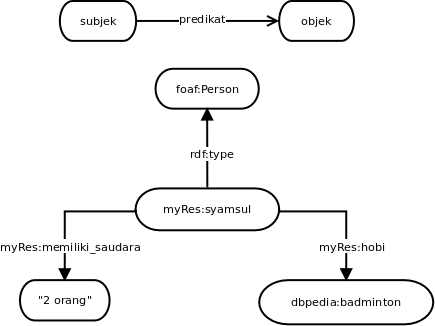
\includegraphics[trim = 29mm 141mm 40mm 0mm, clip, scale=0.6]{gambar}
	\caption{Struktur \emph{statement} RDF}
	\label{fig:rdf_statement}
\end{figure}

Sebagai contoh misalnya pernyataan ``Syamsul hobi badminton'', ``Syamsul memiliki saudara 2 orang'', pernyataan-pernyataan tersebut dapat dibentuk menjadi sebuah \emph{triple}. Pada pernyataan pertama, \emph{Syamsul} adalah merupakan subjek sedangkan \emph{hobi} merupakan sebuah predikat dan \emph{badminton} merupakan sebuah objek, sedangkan pada pernyataan kedua yang menjadi subjek adalah \emph{Syamsul} sedangkan predikat adalah \emph{memmiliki saudara} dan \emph{2 orang} merupakan objek. Jika objek pada pernyataan pertama di atas memerlukan penjelasan lebih lanjut, misalnya mengenai apa itu badminton, maka objek tersebut dapat berupa \emph{resource} dimana \emph{resource} tersebut membentuk triple-triple seperti terlihat pada gambar \ref{fig:rdf_multi_statement}. Pada pernyataan kedua, hanya dimungkinkan berupa literal karena tidak memerlukan penjelasan lebih lanjut mengenai objek itu sendiri.

Agar dapat di proses oleh komputer maka RDF triple harus dituliskan dalam bahasa atau sintak yang dapat dimengerti oleh komputer. Hingga saat ini bentuk penulisan RDF yang direkomendasikan oleh W3C adalah dalam bentuk XML dengan menggunakan namespace yang khusus RDF. Contoh statement di atas dapat kita serialisasi menjadi RDF sebagai berikut:
\lstinputlisting[firstline=1, lastline=7]{./parts/codeblock.xml}
\begin{figure}[!]
	\centering
	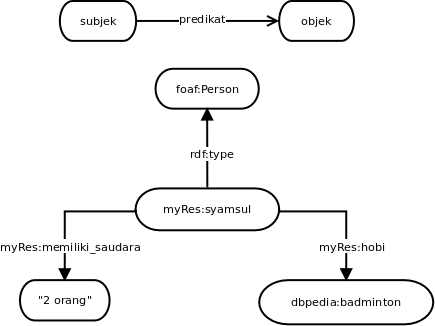
\includegraphics[trim = 0mm 0mm 0mm 93mm, clip, scale=0.55]{gambar}
	\caption{RDF dengan multi-statement}
	\label{fig:rdf_multi_statement}
\end{figure}
Selain XML/RDF, RDF juga dapat dituliskan dengan menggunakan Turtle sintaks sebagai berikut:
\lstinputlisting[firstline=9, lastline=11]{./parts/codeblock.xml}

Sintaks turtle lebih mudah dipahami oleh manusia, sehingga lebih mudah dibentuk. Meskipun sintak ini masih belum menjadi rekomendasi W3C namun besar kemungkinan kedepan juga akan menjadi rekomendasi karena sudah memiliki draft yang dapat dilihat di http://www.w3.org/TR/turtle/.
% \section{\emph{RDF Schema}}
Dalam kasus yang lebih kompleks, RDF tidak cukup kuat untuk menjelaskan semantik dari sebuah subjek yang sedang dijelaskan. Jika kita kembali pada contoh di atas, apabila kita ingin lebih jauh menjelaskan mengenai misalnya apa/siapa Syamsul Muttaqin, RDF tidak dapat menjelaskan hal ini \citep*{antoniou}. Untuk mengatasi hal ini, maka di diperkenalkan RDF Schema (RDFS).

\begin{figure}[h]
	\centering
	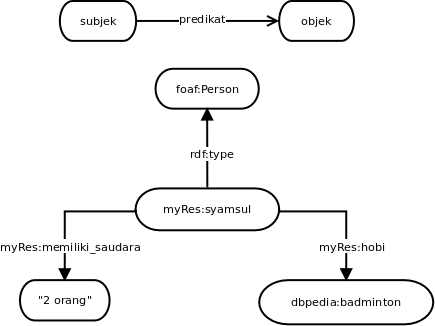
\includegraphics[trim = 0mm 0mm 0mm 32mm, clip, scale=0.55]{gambar}
	\caption{RDFS-statement}
	\label{fig:rdfs_statement}
\end{figure}

Sesuai dengan namanya, RDF Schema memberikan penjelasan lebih jauh mengenai objek yang sedang dibicarakan. Untuk itu RDFS diperkaya dengan beberapa penambahan namespace seperti rdfs:Class yang digunakan untuk menjelaskan tipe dari sebuah objek, rdfs:subClassOf yang merupakan turunan dari kelas, rdfs:domain, rdfs:range, serta beberapa penambahan lainnya. Gambar \ref{fig:rdfs_statement} menunjukkan RDFS statement, dimana \emph{foaf:Person} adalah kelas dan \emph{myRef:syamsul} merupakan \emph{instance} dari kelas \emph{Person}.
\section{OWL Ontologi}
OWL \emph{(Web Ontology Language)} dijadikan sebagai rekomendasi formal oleh W3C pada 10 februari 2004 \citep{liyang_yu}. OWL dirancang untuk kompatibel dengan sintak XML. OWL merupakan pengembangan RDF dan RDFS yang menjadi rekomendasi W3C sebelumnya, oleh karena itu secara sintaksis OWL kompatibel dengan sintak RDF dan RDF Schema.

Ide awal dari pengembangan OWL berdasarkan fakta bahwa RDF Schema belum cukup kuat dalam mereperesentasikan semantik dari sebuah \emph{statement} sehingga diperlukan definisi lebih lanjut. Definisi inilah yang kemudian diperkenalkan dalam OWL. \citet*{antoniou} menjelaskan beberapa model semantik yang tidak dapat dituangkan dalam RDF Schema diantaranya :
\begin{enumerate}
	\item Cakupan \emph{(scope)} dari sebuah properti. Sebagai contoh misalnya properti atau predikat \textit{memakan}, RDFS tidak dapat membatasi range cakupan properti ini hanya untuk kelas tertentu, misalnya kita tidak dapat menyebutkan ``Sapi hanya memakan rumput'', sementara sapi sendiri merupakan \emph{instance} dari kelas binatang, dimana kelas ini tidak hanya berisi sapi saja, namun juga dapat berisi kucing, sementara kucing tidak memakan rumput.
	\item \emph{Disjoint} antar kelas. RDFS hanya menjelaskan mengenai hirarki kelas--sub-kelas, ia tidak dapat membedakan apakah dua atau lebih kelas yang berbeda atau tidak. Sebagai contoh, misalnya kita ingin mendefinisikan kelas mobil dan motor adalah dua kelas yang berbeda, yang artinya apabila \emph{x} adalah instance dari kelas motor, maka \emph{x} tidak mungkin menjadi instance dari kelas mobil. RDFS tidak memiliki properti untuk menjelaskan hal ini, ia hanya dapat menjelaskan bahwa kedua kelas tersebut adalah merupakan sub-kelas dari kelas induk yaitu kendaraan.
	\item Kelas kombinasi. RDFS tidak dapat mendefinisikan sebuah kelas baru yang merupakan gabungan (union) dari dua atau lebih kelas lain. RDFS juga tidak dapat mendefinisikan bentuk kombinasi lain seperti isrisan atau \emph{intersection} ataupun complement dari dua buah kelas yang berbeda. Misalnya kelas Kendaraan adalah gabungan dari kelas Mobil dan Motor.
\end{enumerate}
Sebuah dokumen OWL terdiri dari elemen header, elemen kelas, elemen properti, elemen resktiksi properti, elemen properti khusus, serta elemen kombinasi boolean. 

\subsection{Elemen \emph{header}}
Sesuai dengan standar aturan XML dimana sebuah file terdiri dari sebuah elemen \emph{root}, elemen \emph{root} dari OWL adalah rdf:RDF dimana pada elemen \emph{root} ini dideklarasikan pula beberapa \emph{namspace} yang menjadi standar seperti terlihat pada contoh berikut:
\lstinputlisting[firstline=13, lastline=16]{./parts/codeblock.xml}

Header terdapat diantara elemen \texttt{<owl:Ontology> </owl:Ontology>}. Header berisi informasi mengenai OWL yang bersagkutan seperti informasi versi, keterangan dan lain sebagainya. Berikut ini adalah contoh bentuk dari header OWL
\lstinputlisting[firstline=18, lastline=22]{./parts/codeblock.xml}

\subsection{Elemen kelas}
Bagian selanjutnya adalah elemen kelas, bagian ini berada diantara elemen \texttt{<owl:Class></owl:Class>}. Sebuah kelas dapat terdiri dari beberapa sub kelas, seperti pada RDF Schema, apabila sebuah kelas merupakan sub dari kelas tertentu, maka definisinya dijelaskan di dalam elemen kelas tersebut. Sebagai contoh misalnya definisi kelas berikut:
\lstinputlisting[firstline=24, lastline=27]{./parts/codeblock.xml}

Elemen kelas di atas mendefinisikan sebuah kelas bernama laki-laki yang memiliki hubungan disjoint dengan kelas perempuan dan merupakan sub-kelas dari Person. OWL memiliki beberapa properti kelas selain disjoin seperti equivalentClass yang digunakan untuk menjelaskan ekuivalensi sebuah kelas dengan kelas tertentu, disjointUnion untuk menjelaskan sebuah kelas dijoint dengan beberapa buah kelas yang digabungkan dan lain sebagainya.

\subsection{Elemen properti}
Elemen properti adalah elemen yang menjelaskan mengenai predikat dari sebuah statement, dimana predikat ini menjelaskan hubungan antar kelas atau antar instance sebuah kelas dengan nilai dari properti instance tersebut. Oleh karena itu elemen properti terdiri dari dua jenis yaitu object property dan datatype property.

\emph{Datatype property} menjelaskan hubungan antara \textit{instance} sebuah kelas dengan properti dari \textit{instance} tersebut, misalnya properti \textbf{umur} menjelaskan hubungan antara \textbf{person1} dengan sebuah literal value \textbf{"28"}. 
\lstinputlisting[firstline=29, lastline=31]{./parts/codeblock.xml}

\emph{Object property} menjelaskan hubungan antara sebuah kelas dengan kelas lainnya, misalnya properti diampuOleh menjelaskan hubungan antara kelas dosen dengan kelas matakuliah. 
\lstinputlisting[firstline=33, lastline=37]{./parts/codeblock.xml}

OWL juga memungkinkan kita untuk mendefinisikan inverse dari sebuah properti. Dari contoh di atas, elemen \texttt{<owl:inverseOf rdf:resource="\#mengampu" />} menjelaskan bahwa properti \textbf{diampuOleh} memiliki properti inverse yaitu mengampu, dimana nilai \texttt{rdfs:domain} dan \texttt{rdfs:range} dari properti mengampu merupakan kebalikan dari nilai \texttt{rdfs:domain} dan \texttt{rdfs:range} yang dimiliki oleh properti \textbf{diampuOleh}.

\subsection{Sub-bahasa OWL}
Kemampuan OWL dalam membentuk ekspresi pengetahuan yang sangat lengkap memunculkan kendala dalam hal kemampuan komputer untuk melakukan \emph{reasoning}. Waktu komputasi yang dibutuhkan dalam proses reasoning dapat tidak terhingga, oleh karena itu kelompok kerja bidang ontologi di W3C seperti yang disebutkan oleh \citet*{mcguinness_vanharmelen} membagi OWL ontologi menjadi tiga buah sub bahasa berdasarkan batasan ekspresi logika yang dapat dibentuk yaitu:
\begin{enumerate}
	\item OWL-Full
	\item OWL-DL
	\item OWL-Lite
\end{enumerate}
OWL-Lite merupakan sub-bagian dari OWL-DL, demikian juga dengan OWL-DL merupakan sub-bagian dari OWL-Full. Gambar \ref{fig:owl_subset} menunjukkan ilustrasi dari \emph{subset} OWL.
\begin{figure}[h]
	\centering
	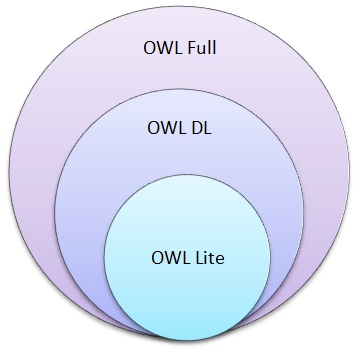
\includegraphics[width=0.5\textwidth]{owl_subset.jpg}
	\caption{Diagram venn \emph{subset} OWL 1}
	\label{fig:owl_subset}
\end{figure}
\section{OWL 2 Ontologi}
OWL terus dikembangkan seiring dengan semakin pesatnya perkembangan dan kebutuhan akan \emph{knowledge sharing}, oleh karena itu, kelompok kerja ontologi di W3C pada tahun 2012 menetapkan versi baru dari OWL yang disebut dengan OWL 2.0 atau OWL 2.

OWL 2 merupakan kelanjutan dari OWL 1.1 dengan beberapa penambahan dan perbaikan fitur. \ref{fig:owl_2_structure} memperlihatkan struktur dasar dari OWL 2.

Bagian atas pada gambar \ref{fig:owl_2_structure} menunjukkan format sintak yang dapat dipergunakan dalam menyusun ontologi dengan menggunakan bahasa OWL 2. Pada OWL 1, format yang dapat digunakan terbatas pada RDF/XML, sedangkan pada OWL 2 seperti yang terlihat dalam gambar \ref{fig:owl_2_structure} terdapat lima buah format yang dapat digunakan. Dari semua format tersebut, W3C hanya mewajibkan format RDF/XML sebagai format standar, sedangkan format lainnya berupa opsional saja.

\begin{figure}[h]
	\centering
	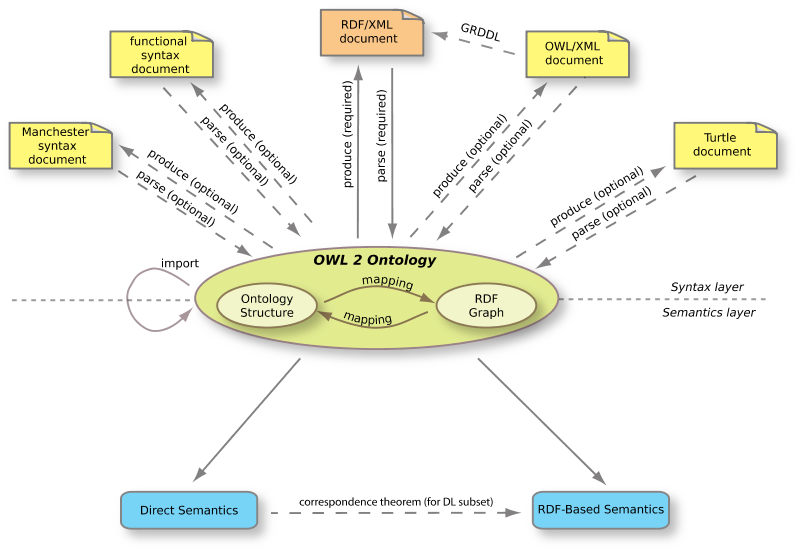
\includegraphics[width=1\textwidth]{owl_2_structure}
	\caption{Struktur OWL 2.0}
	\label{fig:owl_2_structure}
\end{figure}

Masing-masing format sintak memiliki kelebihan dan kekurangan. Format RDF/XML memiliki dukungan yang paling baik, hanya saja kurang intuitif jika dibandingkan dengan Turtle, Functional maupun Manchester, sedangkan Turtle Functional dan Manchester tidak memiliki dukungan \emph{tool} yang baik.
\begin{itemize}
	\item contoh sintak RDF/XML \\
	\begin{lstlisting}
		<SubClassOf>
			<Class IRI="Woman"/>
			<Class IRI="Person"/>
		</SubClassOf>
	\end{lstlisting}

	\item contoh sintak functional \\
	\begin{lstlisting}
		SubClassOf( :Woman :Person )
	\end{lstlisting}
	
	\item contoh sintak manchester
	\begin{lstlisting}
		Class: Woman
			SubClassOf: Person
	\end{lstlisting}

	\item contoh sintak turtle
		\begin{lstlisting}
			:Woman rdfs:subClassOf :Person .
		\end{lstlisting}
\end{itemize}

\subsection{Profil OWL 2}
Seperti yang telah dijelaskan sebelumnya bahwa OWL 1 memiliki tiga sub-bahasa, namun dalam praktiknya ketiga sub-bahasa tersebut ternyata belum cukup untuk memenuhi kebutuhan yang ada. \citet{patel} mengungkapkan beberapa permasalahan dalam \emph{real world application} yang diadapi para pengembang.

Berdasarkan fakta tersebut, maka OWL 2 membagi sub-bahasa kedalam tiga bagian yaitu:
\begin{itemize}
	\item OWL 2 EL
	\item OWL 2 QL
	\item OWL 2 RL
\end{itemize}

Masing-masing profil dibatasi oleh batasan sintaks \emph{(syntactic restriction)}. Perlu diketahui bahwa sub-bahasa OWL 2 ini berdasarkan pada OWL-DL, sehingga semua ekspresi yang diyatakan valid pada OWL 2 EL misalnya, secara otomatis akan valid juga untuk OWL-DL. Gambar \ref{fig:owl_2_profile} menunjukkan diagram venn relasi antar sub-bahasa pada OWL 2.

\begin{figure}[h]
	\centering
	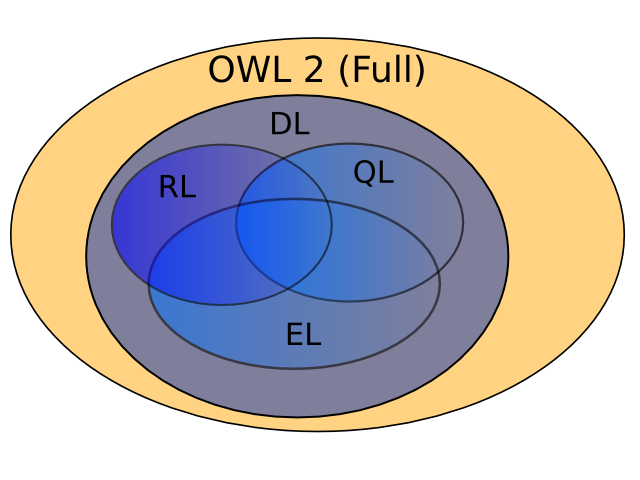
\includegraphics[scale=0.4]{owl_2_profile}
	\caption{Diagram venn profil OWL 2}
	\label{fig:owl_2_profile}
\end{figure}
\section{Ontologi Reasoning}
Proses \emph{reasoning} adalah proses untuk mendapatkan \emph{statement} yang terdapat dalam ontologi namun tidak dinyatakan secara implisit. \citet*{antoniou} menyebutkan beberapa hal yang dapat dihasilkan melalui proses reasoning adalah:
\begin{itemize}
	\item Keanggotaan kelas \emph{(class membership)}. Menentukan apakah sebuah \emph{instance} merupakan anggota dari sebuah kelas. Penentuan keanggotaan ini dilakukan dengan cara memeriksa properti yang dimiliki oleh \emph{instance} tersebut.
	\item Klasifikasi . Apabila terdapat kelas bebek yang merupakan sub-kelas motor dan kelas motor sub-kelas dari kendaraan, maka dapat diperoleh \emph{statement} bahwa kelas bebek adalah sub-kelas dari kendaraan.
	\item Konsistensi dari sebuah ontologi. Untuk menentukan apakah sebuah ontologi konsisten seacara logika dapat pula dilakukan dengan menggunakan proses rasoning. Sebagai contoh, misalnya terdapat dua buah kelas mahasiswa dan dosen yang dinyatakan \emph{disjoint} dan terdapat satu buah \emph{instance} syamsul yang merupakan anggota dari kelas dosen dan mahasiswa, maka ontologi tersebut dikatakan tidak konsisten.
	\item Kesetaraan kelas \emph{equivalence of classes}. Reasoning juga dapat digunakan untuk menentukan ekivalensi kelas, misalnya terdapat kelas kajur yang dinyatakan ekivalen dengan kelas karyawan dan kelas karyawan ekivalen dengan dosen, maka kelas kajur dengan dosen juga ekivalen. 
\end{itemize}
\section{Ontology Merging}
\section{\textit{Question Answering}}
Semakin banyaknya sumber informasi yang tersedia di internet menyebabkan semakin sulitnya mendapatkan infromasi yang relevan, informasi yang diberikan oleh mesin pencari konvensional saat ini hanya berupa tautan ke laman yang mengandung meta-keyword yang mirip dengan kata kunci yang dimasukkan, pengguna harus membaca terlebih dahulu laman web yang diberikan oleh mesin pencari yang tentu saja akan membutuhkan waktu. Hal ini menjadi tidak efisien terutama apabila yang akan dicari adalah informasi-informasi sederhana seperti informasi cuaca, alamat sebuah instansi dan lain sebagainya. 

Tujuan dari \emph{Question Answering (QA)} adalah untuk mencari jawaban atas pertanyaan pengguna dalam bentuk terstruktur maupun tidak terstruktur \citep*{moussa_kader}. Pengguna memasukkan pertanyaan dalam bentuk bahasa alami, sistem kemudian akan memproses pertanyaan dan akan menyajikan jawabannya dalam bentuk jawaban singkat hasil pemrosesan.

\citet*{ramprasath_hariharan} menyebutkan arsitektur sebuah sistem QA secara umum terdiri dari beberapa modul yiatu :
\begin{enumerate}
	\item Antarmuka pertanyaan \emph{(Query Interface)} \\
		Modul ini berfungsi sebagai penjembatan antara pengguna dengan sistem. Di sinilah pengguna memasukkan kata kunci pencariannya dalam bentuk bahasa alami.
	\item Modul Analisa Pertanyaan \emph{(Query Analyzer)} \\
		Modul ini akan menganalisa subjek, predikat dan objek dari kata kunci yang dimasukkan oleh pengguna.
	\item Modul Klasifikasi Pertanyaan \emph{(Question Classification)} \\
		Bagian ini berfungsi untuk memeriksa tipe dari pertanyaan seperti misalnya \emph{siapa} secara eksplisit menanyakan tentang orang, \emph{kapan}, berhubungan dengan waktu dan lain sebagainya. Klasifikasi ini akan digunakan sebagai pegangan pada tahapan validasi jawaban, apakah jawaban yang diberikan sesui dengan pertanyaan.
	\item Pembentukan Query \emph{(Query Reformulation)} \\
		Modul ini memegang peranan cukup penting, karena bagian ini yang bertanggungjawab atas keabsahan jawaban yang dihasilkan.
	\item Modul Pencari \emph{(Search Engine)} \\ 
		Modul ini digunakan untuk mencari jawaban dari pertayaan yang dihasilkan oleh modul query reformulation. Jawaban akan dicari pada sumber pengetahuan yang telah ditetukan, misalnya laman web ataupun modul basis pengetahuan tertentu seperti ontologi dan lain sebagainya.
	\item Module Ekstraksi \emph{(Answering Extractor)} \\ 
		Kandidat jawaban yang dihasilakan oleh modul search engine kemudian akan dikirimkan ke bagian ini, dimana kandidat jawaban yang umumnya berupa dokumen akan diekstraksi dan selanjutkan akan dikirimkan ke modul penyaring.
	\item Modul Penyaring Jawaban \emph{(Answer Filtering)} \\
		Modul ini akan menyaring kandidat jawaban hasil ekstraksi yang relevan dengan pertanyaan yang diberikan.
	\item Validasi Jawaban \emph{(Answer Validation)} \\ 
		Sebelum jawaban ditampilkan kepada pengguna, terlebih dahulu jawaban akan divalidasi berdasarkan klasifikasi pertanyaan yang telah ditentukan pada modul klasifikasi pertanyaan.
	\item Ontology Merging \\
		Mesikipun multi-ontologi memiliki kelebihan pada kayanya konsep pengetahuan yang didapat namun demikian oleh karena sangat dimungkinkan masing-masing ontologi yang menjadi sumber informasi ini memiliki struktur yang berbeda, sehingga arsitektur multi-ontologi seperti ini memunculkan tantangan baru yaitu bagaimana menggali informasi dari berbagi ontologi yang tersebar tersebut. Salah satu solusinya adalah dengan menggunakan metode merging.
\end{enumerate}
\citet*{choi} mendefinisikan ontology-merging sebagai proses pembentukan sebuah ontologi yang mendefinisikan sebuah makna tertentu dari dua buah atau lebih ontologi yang mendefinisikan makna tersebut dengan cara dan bahasa yang berbeda, sehingga diharapkan akan terbentuk sebuah ontologi yang memiliki keseragaman bahasa untuk sebuah konsep tertentu. Ontologi hasil merging memiliki menyimpan informasi dari masing-masing ontologi sumber, namun memiliki keunikan dan bukan merupakan pengganti dari ontologi sumber infromasinya.
\chapter{ANALISIS DAN RANCANGAN SISTEM}
\section{Deskripsi Sistem}
Sesuai dengan tujuan awal dari penelitian ini yaitu untuk membangun sistem \emph{question answering} data kabutapen di propinsi Nusa Tenggara Barat maka sistem akan dibangun berbasis web sehingga nantinya dapat diakses secara luas.

Halaman beranda terdiri dari form untuk melakukan input pertanyaan dalam bahasa Indonesia baku yang sesuai dengan tata tulis bahasa Indonesia dan tombol untuk submit pertanyaa, kemudian sistem akan menampilkan jawaban pada halaman yang sama tanpa berpidah halaman, hal ini dimaksudkan untuk menyederhanakan interaksi pengguna dengan sistem. 

Secara umum, sistem \emph{question answering} yang akan dibangun terdiri dari tiga tahapan utama yaitu proses awal, proses utama dan proses akhir. Proses awal berkaitan dengan pemrosesan kalimat tanya dimana proses ini merupakan proses transformasi bahasa alami menjadi pohon urai \emph{(parse tree)} sehingga nantinya komputer dapat memahami maksud dari pertanyaa.

Proses utama merupakan proses pencarian jawaban atas pertanyaan ke dalam ontologi. Proses ini dilakukan dengan cara mengubah pohon urai yang sudah dibentuk pada proses awal menjadi statement query SPARQL-DL yang kemudian dijalankan oleh \emph{query engine}, sedangkan poses akhir adalah proses pembentukan template jawaban yang akan ditampilkan di browser.

Pembentukan pohon urai diawali dengan proses POS Tagging dengan tujuan untuk menandai kelas kata. Proses POS Tagging dilakukan dengan cara melakukan pengecekan ke dalam database lexicon, apabila kelas kata tidak ditemukan, maka proses dilanjutkan dengan proses analisa morfologi untuk menebak kelas kata.


\section{Arsitektur Sistem}
Arsitektur sistem yang akan dibangun ditunjukkan pada gambar \ref{fig:arsitektur_sistem}. Komunikasi antara \textit{client} dengan server untuk proses pencarian data dilakukan secara asinkoron dengan menggunakan AJAX \textit{(Asynchronous Javascript and XML)}. Masing-masing ontologi yang akan dibangun diletakkan di lokasi yang terpisah yang nantinya dapat diakses melalui protokol http.

\begin{figure}[h]
    \centering
    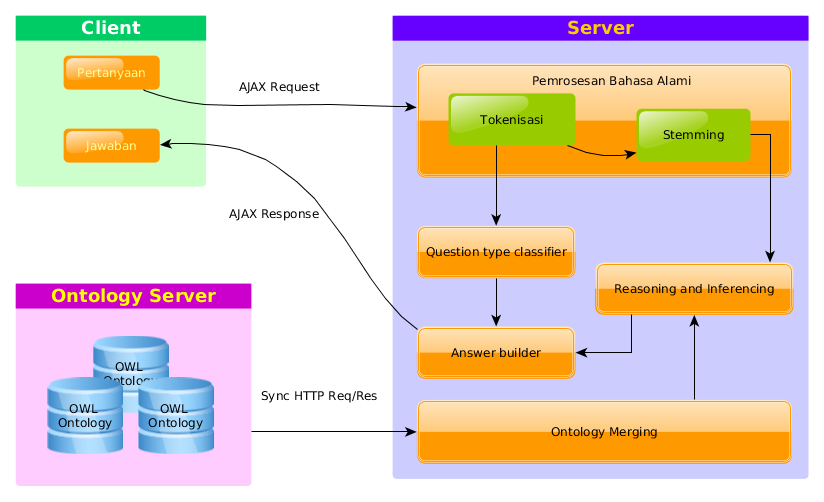
\includegraphics[width=1\textwidth]{arsitektur_sistem}
    \caption{Arsitektur sistem yang akan dikembangkan}
    \label{fig:arsitektur_sistem}
\end{figure}
\section{Perancangan Sistem}
Sistem \emph{question answering} yang akan dibangun menggunakan platform Java dengan metode pemrograman berorientasi objek, untuk itu pemodelan sistem menggunakan bahasa UML \emph{(Unified Modelling Language)}. Adapun diagram UML yang digunakan untuk merepresentasikan sistem adalah \emph{usecase diagram, activity diagram, sequence diagram dan state diagram}. 

\subsection{Diagram \emph{usecase}}
Diagram \emph{usecase} digunakan untuk menunjukkan interaksi sistem dengan aktor atau pengguna, berapa jumlah aktor serta hak akses masing-masing aktor terhadap sistem. Gambar \ref{fig:usecase_diagram} menunjukkan hubungan antara aktor dengan sistem. Sistem \emph{question answering} yang akan dibangun hanya melibatkan satu aktor yaitu pengguna yang akan memasukkan pertanyaan.
\begin{figure}[h]
    \centering
    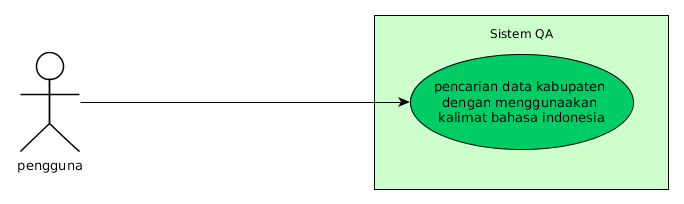
\includegraphics[width=0.8\textwidth]{usecase_diagram}
    \caption{Diagram \emph{usecase} sistem \emph{question answering}}
    \label{fig:usecase_diagram}
\end{figure}

\subsection{Diagram kelas}
Sistem \emph{question answering} yang akan dikembangkan memiliki beberapa kelas yang dibagi ke dalam beberapa paket utama yaitu paket controllers, models dan helpers.

\subsubsection{Kelas \emph{Main}}
Kelas \emph{Main} merupakan kelas yang berfungsi sebagai \emph{controller} yang bertugas untukmengatur komunikasi antara \emph{client} dengan server. Kelas ini merupakan sub kelas dari httpServlet. Kelas \emph{Main} diletakkan dalam paket \emph{controller} sedangkan kelas httpServlet berada pada paket \emph{javax.servlet.http}

Kelas Main terdiri dari dua buah method yaitu \emph{doGet()} dan \emph{processRequest()}. \emph{doGet()} memiliki akses kenampakan \emph{protected} dan merupakan versi \emph{overriding} dari method \emph{doGet()} pada kelas httpServlet. Method \emph{processRequest()} memiliki akses kenampakan private sehingga tidak dapat diakses dari luar atau dari web karena method ini hanya berfungsi sebagai pemroses internal yang hanya akan dipanggil melalui internal kelas Main.

\subsubsection{Kelas Tokenizer}
Tokenizer merupakan kelas yang berfungsi untuk melakukan proses tokenisasi terhadap kalimat tanya yang dikirimkan oleh user. Tokenizer akan menghasilkan data token berupa \emph{array list}
\subsubsection{Kelas NGram}
Kelas ini berfungsi untuk melakukan proses penggabungan kata per kata untuk kemudian di cek pada ontologi apakah kata yang terbentuk terdapat di dalam ontologi atau tidak. Kelas ini juga berfungsi untuk melakukan POS-Tangging terhadap token untuk menandakan tipe dari kata tersebut.

Kelas NGram memiliki tiga buah method yaitu konstruktor, \emph{processNgram()} dan \emph{getNgram()}. method konstruktor menerima input berupa array list token sedangkan method \emph{processNgram()} tidak memiliki masukan maupun kembalian, method ini hanya digunakan untuk melakukan proses ngram secara internal, oleh karena itu kenampakannya dibuat \emph{private}. Method \emph{getNgram()} memiliki kenampakan public dengan kembalian berupa array list yang berisi string kata yang telah diberikan tag.

\subsubsection{Kelas Ontology}
Kelas Ontology merupakan kelas yang berfungsi untuk melakukan inisiasi ontologi. Kelas ini juga berfungsi untuk melakukan proses \emph{merging} terhadap ketiga ontologi sumber yang sudah di load sebelumnya.


\begin{figure}[h]
    \centering
    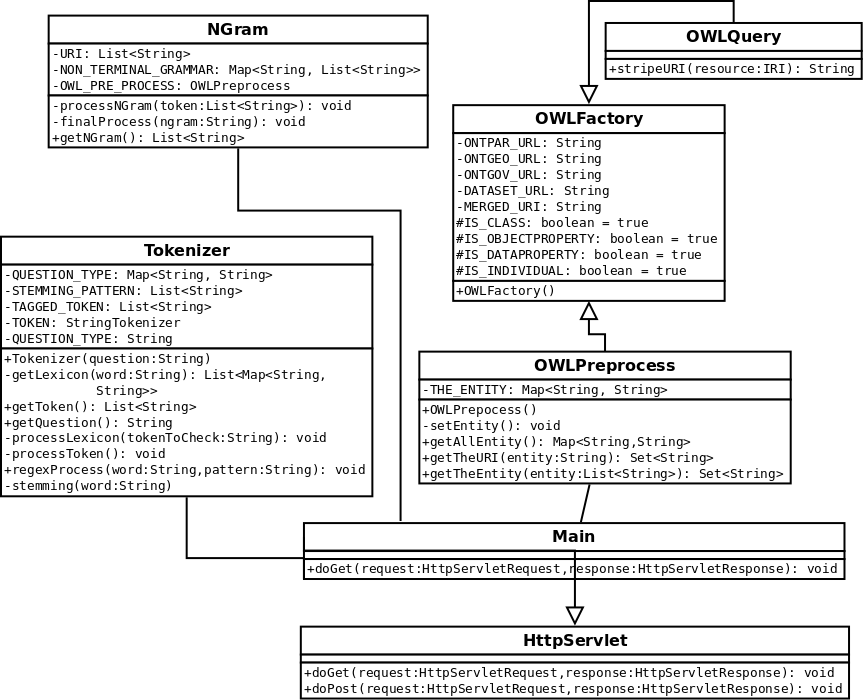
\includegraphics[width=1\textwidth]{class_diagram}
    \caption{Diagram kelas aplikasi}
    \label{fig:class_diagram}
\end{figure}

\subsection{Diagram \emph{activity}}
\subsection{Diagram \emph{sequence}}
\section{Perancangan Antar Muka Aplikasi}
Aplikasi \emph{question answering} yang akan dikembangkan dalam penelitian ini hanya memiliki satu buah halaman antar seperti terlihat pada gambar \ref{fig:rancangan_antarmuka}. Masukan pertanyaan dan jawaban diletakkan dalam satu buah halaman yang sama. Pada tahap awal sebelum pengguna mengirimkan pertanyaan hanya akan disediakan sebuah \emph{field} dengan tipe \emph{text} dan sebuah tombol submit yang berfungsi untuk mengirimkan pertanyaan ke sever.

\begin{figure}[h]
    \centering
    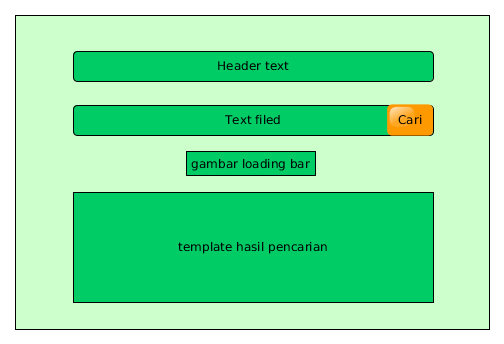
\includegraphics[width=1\textwidth]{rancangan_antar_muka}
    \caption{Rancangan antar muka aplikasi \emph{question answering} data kabupaten di Nusa Tenggara Barat}
    \label{fig:rancangan_antarmuka}
\end{figure}

Bagian header berisi nama dari aplikasi \emph{question answering}, kemudian dibawahnya terdapat sebuah text field yang digunakan untuk memasukkan pertanyaan. Atribut \emph{placeholder} dari input field diisi dengan tulisan ``Masukkan pertanyaan'' untuk memudahkan pengguna memahami bagian input field itu sendiri. Selanjutnya, di sebelah input filed terdapat sebuah tombol yang digunakan untuk melakukan submit form.

Bagian bawah input form diletakkan sebuah gambar ``loading bar'' yang berfungsi untuk memberitahuan kepada user bahwa proses pencarian jawaban sedang berlangsung. Gambar ini akan muncul ketika pengguna telah melakukan submit form dengan cara menekan tombol ``cari'' atau dengan menekan tombol ``enter'' pada keyboard. Setelah jawaban diperoleh, maka gambar tersebut akan secara otomatis hilang dan jawaban hasil pencarian akan ditampilkan dibawahnya. Setelah jawaban ditampilkan, input filed tidak akan dikosongkan, hal ini dimaksudkan agar pengguna dapat melihat relasi antara pertanyaan yang dimasukkan dengan hasil jawaban yang didapatkan.

Pengguna dapat melakukan pencarian baru dengan cara menghapus pertanyaan sebelumnya yang terdapat pada input field untuk kemudian menggantinya dengan pertanyaan yang baru. Sesaat setelah user menekan tombol ``enter'' atau tombol ``cari'' maka bagian template hasil pencarian akan dikosongkan dan gambar ``loading bar'' akan kembali muncul seperti pada proses sebelumnya.
\section{Perancangan Ontologi}
Sistem yang akan dibangun ini nantinya akan mengguakan tiga buah ontologi yang berbeda, masing-masing ontologi dapat diakses sercara terpisah melalui protokol http.

\emph{Term} yang akan digunakan untuk membangun ketiga ontologi ini mengacu pada \emph{term} yang telah tersedia pada dbpedia versi bahasa Indoensia. Apabila terdapat \emph{term} yang tidak ada dalam dbpedia, maka akan dibangun term sendiri dengan menggunakan \emph{namespace} http://www.ntbprov.go.id/resource/<nama\_term>. Format pembuatan <nama\_term> mengacu pada sistem penamaan \emph{resource} pada dbpedia.

\subsection{Ontologi pariwisata}
Ontologi pariwisata secara spesifik menyimpan fakta-fakta mengenai informasi pariwisata dari masing-masing kabupaten dan kota. Ontologi ini diberi nama ntbpar.owl. Kelas serta properti yang terdapat dalam ontologi ntbpar.owl ditunjukkan pada tabel \ref{table:ontopar_class}

\begin{table}[!]
	\caption{Daftar kelas dalam ontologi pariwisata}
	\label{table:ontopar_class}
	\begin{tabularx}{\textwidth}{|c|X|X|}
		\hline
		No & Nama Kelas & Keterangan \\
		\hline
		1 & Bar & - \\
		\hline
		2 & Budaya & - \\
		\hline
		3 & Desa & - \\
		\hline
		4 & Hotel & - \\
		\hline
		5 & Losmen & - \\
		\hline
		6 & Villa & - \\
		\hline
		7 & Kerajinan & - \\
		\hline
		8 & Kuliner & - \\
		\hline
		9 & Makanan & - \\
		\hline
		10 & Minuman & - \\
		\hline
		11 & Pariwisata & - \\
		\hline
		12 & Desa\_wisata & - \\
		\hline
		13 & Desa\_adat & - \\
		\hline
		14 & Ekowisata & - \\
		\hline
		15 & Wisata\_alam & - \\
		\hline
		16 & Air\_terjun & - \\
		\hline
		17 & Gili & - \\
		\hline
		18 & Pulau & - \\
		\hline
		19 & Gunung & - \\
		\hline
		20 & Pantai & - \\
		\hline
		21 & Wisata\_budaya & - \\
		\hline
		22 & Restoran & - \\
		\hline
		23 & Spa & - \\
		\hline
	\end{tabularx}
\end{table}

\subsection{Ontologi geografi}
Ontologi geografi secara spesifik menyimpan fakta-fakta mengenai informasi geografis dari masing-masing kabupaten dan kota. Kelas serta properti yang terdapat pada ontologi ini ditunjukkan dalam tabel \ref{table:ontogeo_class}

\begin{table}[!]
	\caption{Daftar kelas ontologi geografi}
	\label{table:ontogeo_class}
	\begin{tabularx}{\textwidth}{|c|X|X|}
		\hline
		No & Nama Kelas & Keterangan \\
		\hline
		1 & Desa & - \\
		\hline
		2 & Ibu\_kota & - \\
		\hline
		3 & Kabupaten & - \\
		\hline
		4 & Kecamatan & - \\
		\hline
		5 & Komoditas & - \\
		\hline
		6 & Perikanan & - \\
		\hline
		7 & Perkebunan & - \\
		\hline
		8 & Pertambangan & - \\
		\hline
		9 & Pertanian & - \\
		\hline
		10 & Kota & - \\
		\hline
		11 & Provinsi & - \\
		\hline
	\end{tabularx}
\end{table}

\subsection{Ontologi Pemerintahan}
Ontologi pemerintahan atau ontogov.owl secara spesifik menyimpan fakta-fakta mengenai informasi pemerintahan di tingkat kabupaten, termasuk dinas, kecamatan dan desa. Daftar kelas serta properti yang terdapat dalam ontologi ini ditunjukkan dalam tabel \ref{table:ontogeo_class}

\begin{table}[!]
	\caption{Daftar kelas ontologi pemerintahan}
	\label{table:ontogov_class}
	\begin{tabularx}{\textwidth}{|c|X|X|}
		\hline
		No & Nama Kelas & Keterangan \\
		\hline
		1 & Organization & - \\
		\hline
		2 & Pemerintah\_daerah & - \\
		\hline
		3 & Badan & - \\
		\hline
		4 & Biro & - \\
		\hline
		5 & Desa & - \\
		\hline
		5 & Dinas & - \\
		\hline
		7 & Kabupaten & - \\
		\hline
		8 & Kecamatan & - \\
		\hline
		9 & Kota & - \\
		\hline
		10 & Provinsi & - \\
		\hline
		11 & Person & - \\
		\hline
		12 & Bupati & - \\
		\hline
		13 & Gubernur & - \\
		\hline
		14 & Kepala\_desa & - \\
		\hline
		15 & Pegawai\_negeri & - \\
		\hline
		16 & PNS & - \\
		\hline
		17 & Camat & - \\
		\hline
		18 & Kepala\_badan & - \\
		\hline
		19 & Kepala\_biro & - \\
		\hline
		20 & Kepala\_dinas & - \\
		\hline
		21 & Wakil\_camat & - \\
		\hline
		22 & Wakil\_bupati & - \\
		\hline
		23 & Wakil\_gubernur & - \\
		\hline
		24 & Wakil\_wali\_kota & - \\
		\hline
		25 & Wali\_kota & - \\
		\hline
	\end{tabularx}
\end{table}
\chapter{IMPLEMENTASI}
\section{Implementasi Ontologi}
Rancangan ontologi yang telah dijelaskan pada bab sebelumnya akan diimlementasikan pada bab ini. Implementasi rancangan ontologi dilakukan dengan bantuan perangkat lunak Protege versi 5. OWL API versi 4 yang digunakan dalam penelitian ini telah mendukung berbagai macam format serialisasi, salah satu diantaranya adalah Manchester Syntax, oleh karena itu implementasi ketiga ontologi yang akan digunakan pada penelitian ini akan menggunakan Manchester syntax. Manchester syntax dipilih dengan tujuan agar struktur ontologi mudah dipahami.

Implementasi ontologi pariwisata ditunjukkan pada gambar \ref{fig:ntbpar_class}
\begin{figure}[h]
	\centering
	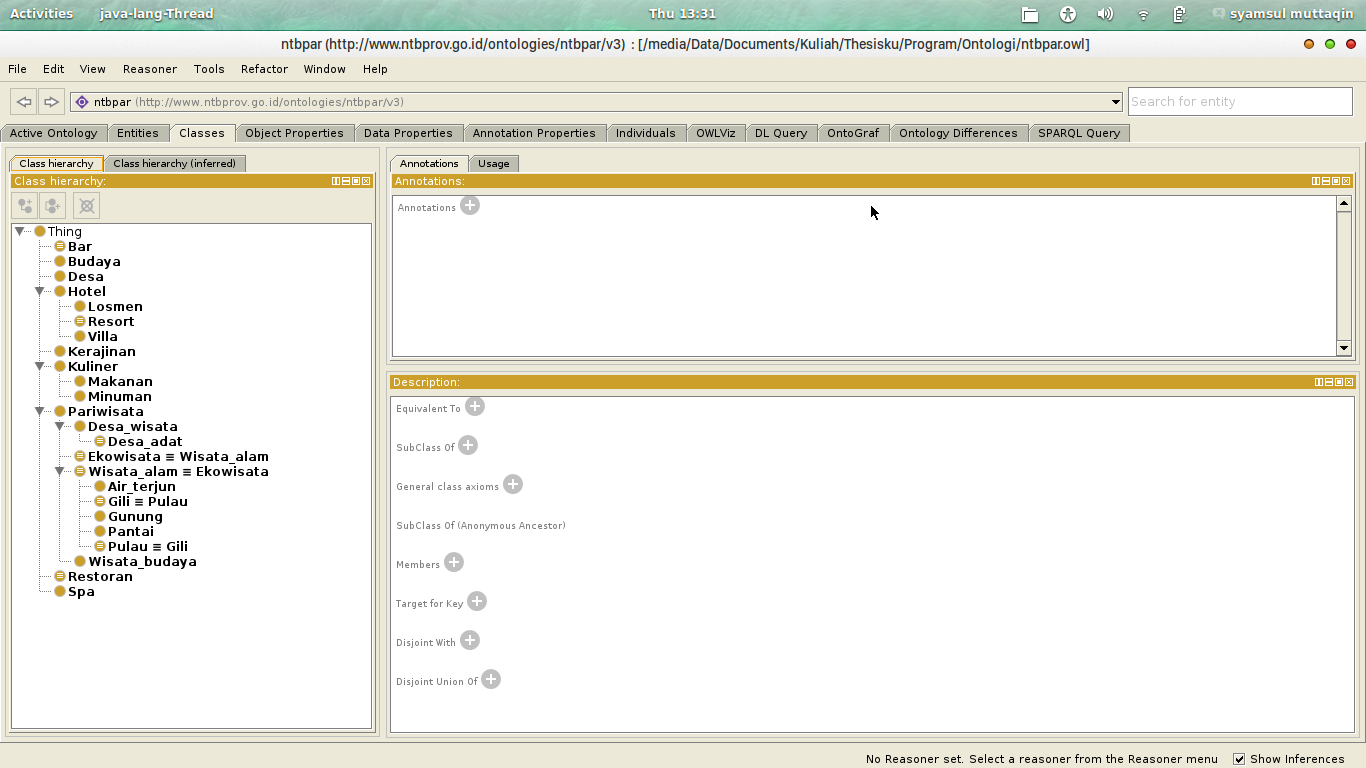
\includegraphics[width=1\textwidth]{ntbpar_class}
	\caption{Implementasi kelas pada ontologi pariwisata}
	\label{fig:ntbpar_class}
\end{figure}

\begin{figure}[h]
	\centering
	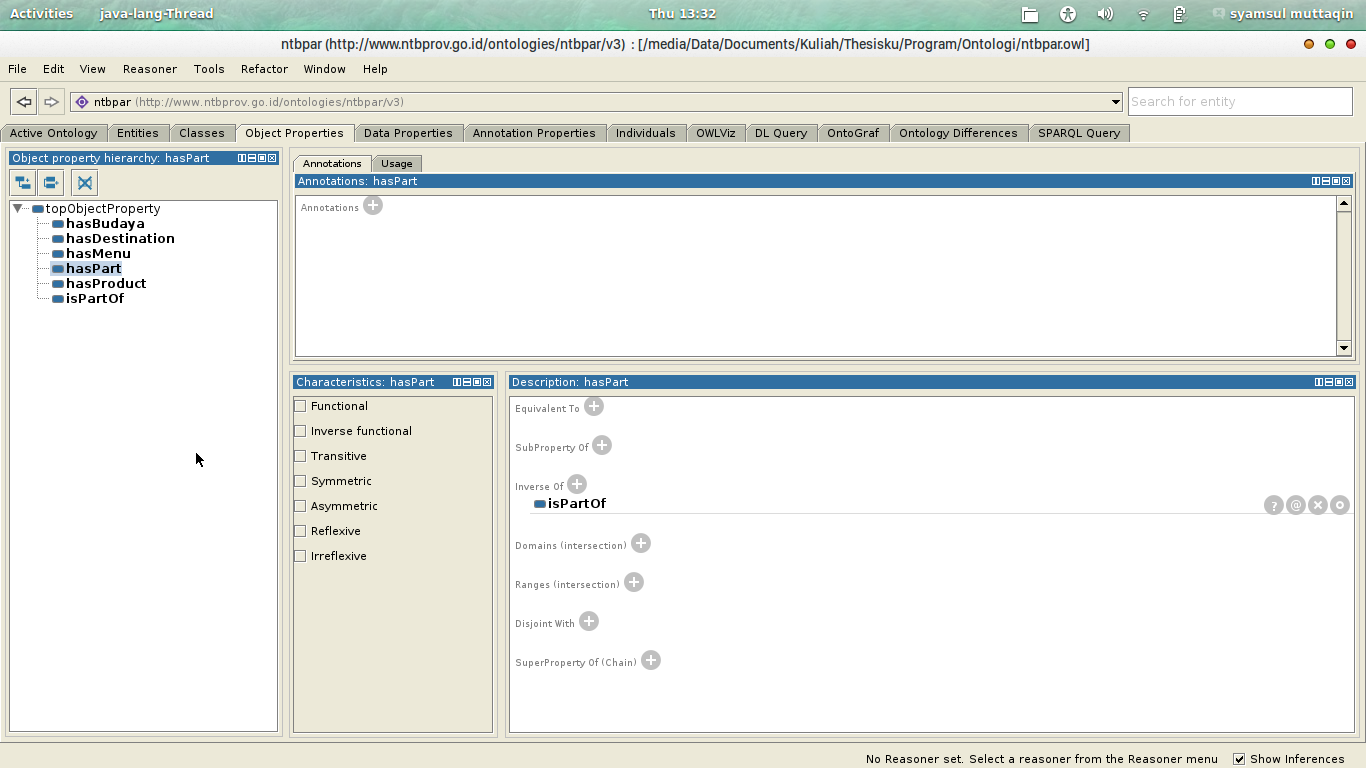
\includegraphics[width=1\textwidth]{ntbpar_op}
	\caption{Implementasi objek properti pada ontologi pariwisata}
	\label{fig:ntbpar_op}
\end{figure}

\begin{figure}[h]
	\centering
	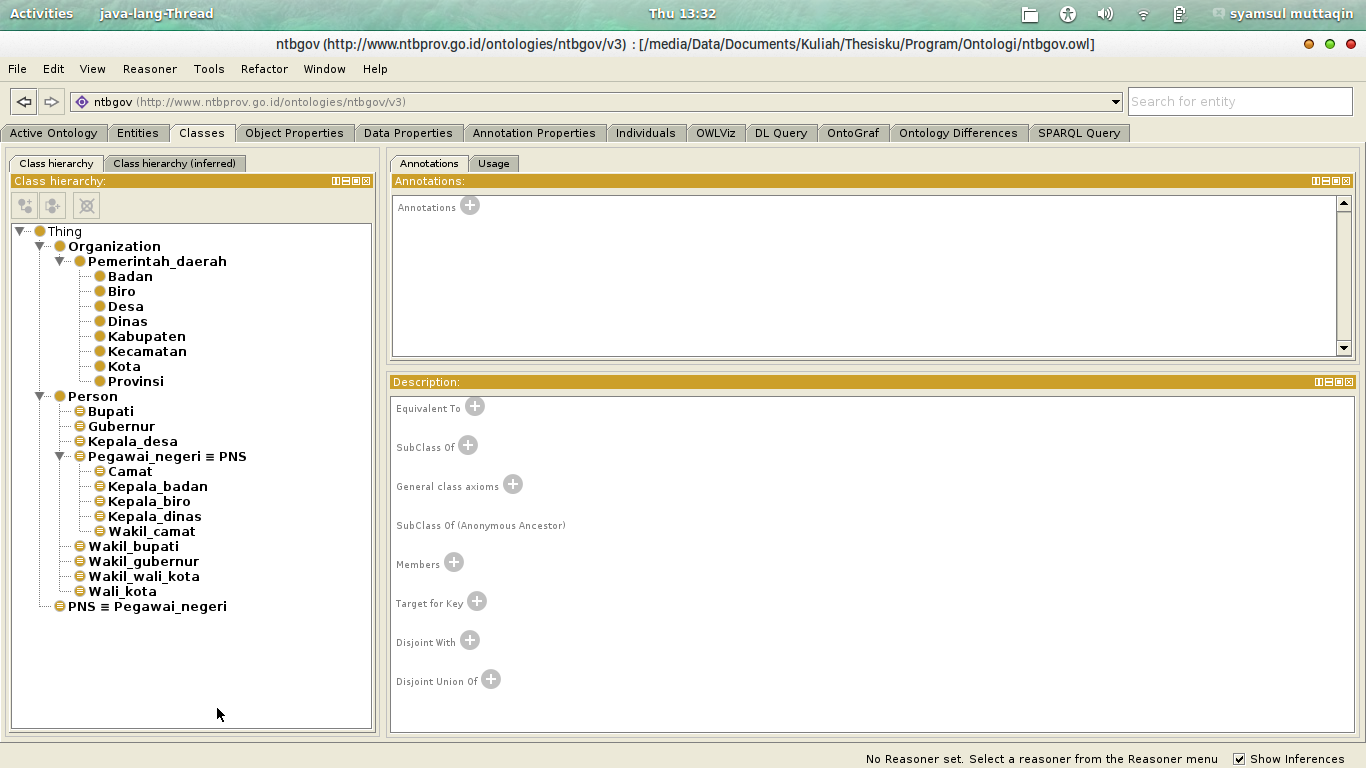
\includegraphics[width=1\textwidth]{ntbgov_class}
	\caption{Implementasi kelas pada ontologi pemerintahan}
	\label{fig:ntbgov_class}
\end{figure}

\begin{figure}[h]
	\centering
	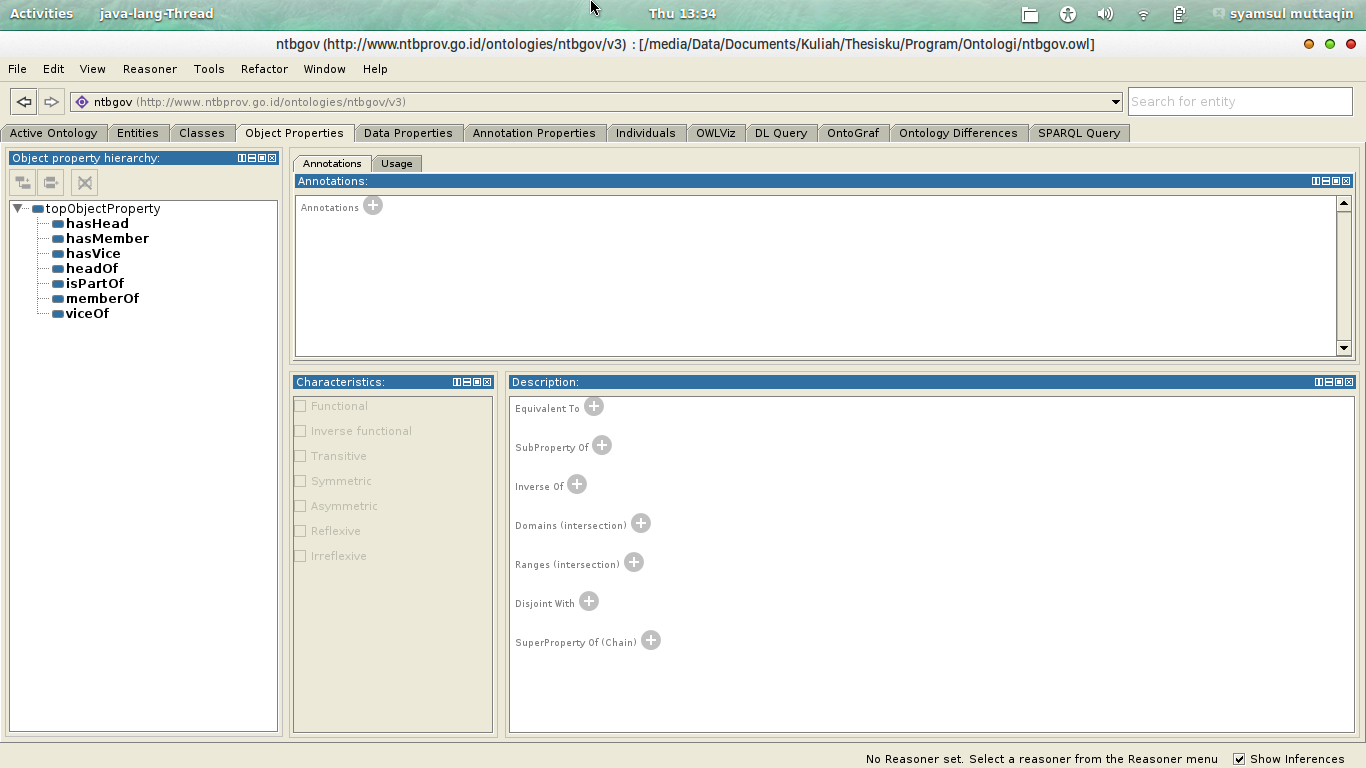
\includegraphics[width=1\textwidth]{ntbgov_op}
	\caption{Implementasi objek properti pada ontologi pemerintahan}
	\label{fig:ntbgov_op}
\end{figure}

\begin{figure}[h]
	\centering
	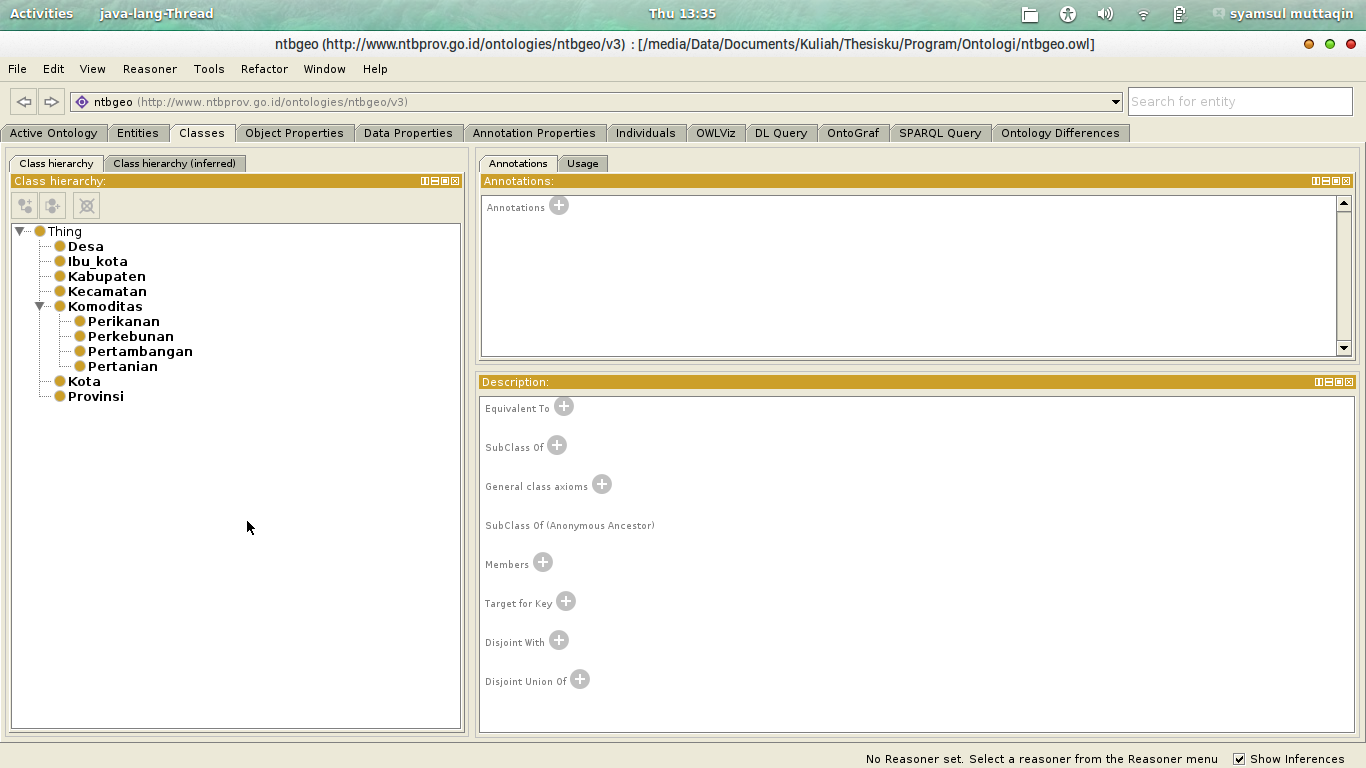
\includegraphics[width=1\textwidth]{ntbgeo_class}
	\caption{Implementasi kelas pada ontologi geografi}
	\label{fig:ntbgeo_class}
\end{figure}

\begin{figure}[h]
	\centering
	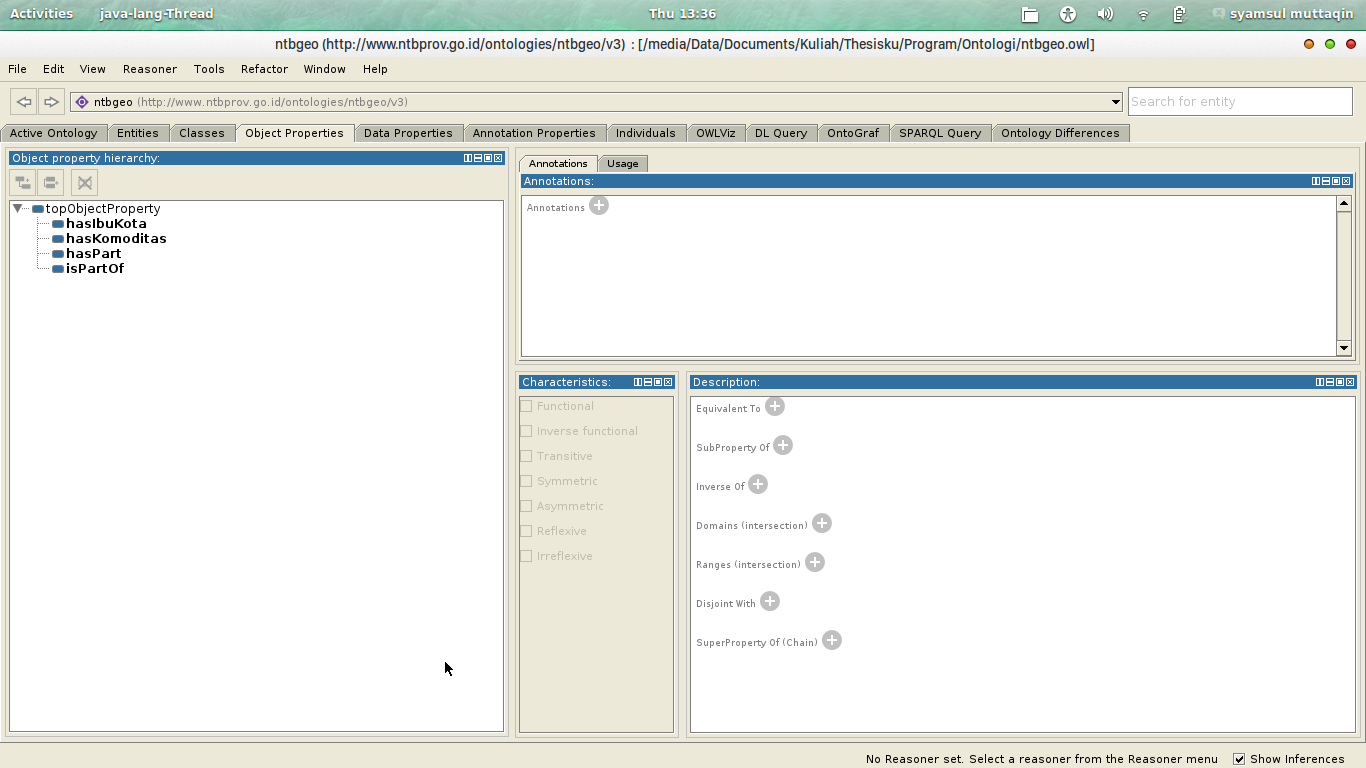
\includegraphics[width=1\textwidth]{ntbgeo_op}
	\caption{Implementasi objek properti pada ontologi geografi}
	\label{fig:ntbgov_op}
\end{figure}

\begin{landscape}
\begin{figure}[h]
	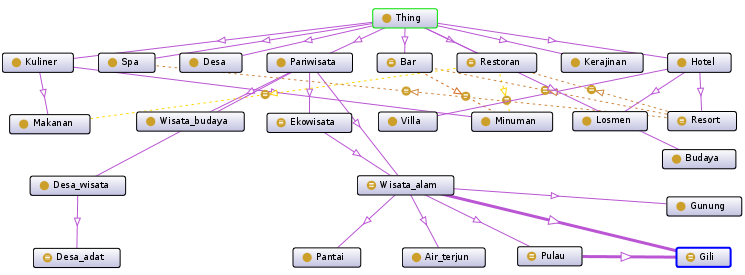
\includegraphics[scale=0.8]{ntbpar}
	\caption{Struktur ontologi pariwisata}
	\label{fig:struktur_ntbpar}
\end{figure}
\end{landscape}

\begin{figure}[h]
	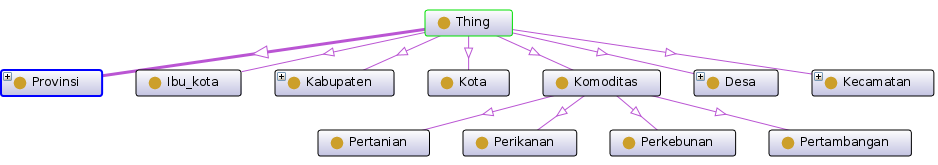
\includegraphics[width=\textwidth]{ntbgeo}
	\caption{Struktur ontologi geografi}
	\label{fig:struktur_ntbgeo}
\end{figure}

\begin{landscape}
	\begin{figure}[h]
		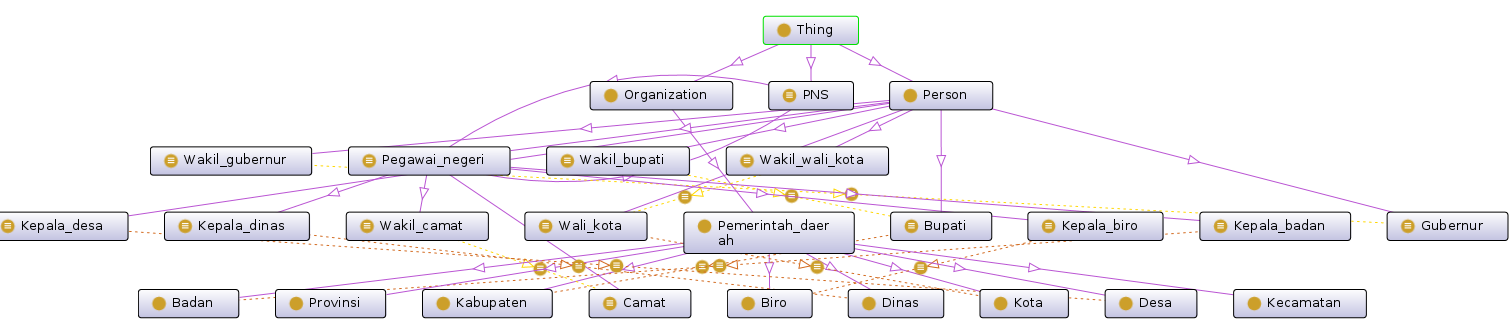
\includegraphics[scale=0.45]{ntbgov}
		\caption{Struktur ontologi pemerintahan}
		\label{fig:struktur_ntbgov}
	\end{figure}
\end{landscape}
\section{Implemenatasi Sistem}
Implemetasi hasil rancangan sistem dilakukan dalam dua tahapan utama, yaitu implementasi pemrosesan bahasa sebagai masukan dan implementasi pembangunan ontologi sebagai sumber pengetahuan sistem.

\subsection{Pembentukan token}
\section{Implementasi Antar Muka Aplikasi}
% \chapter{HASIL PENELITIAN DAN PEMBAHASAN}
\section{Skenario Pengujian}
Pengujian terhadap sistem \emph{question answering} yang dikembangkan dalam penelitian ini meliputi pengujian sistem secara umum dan pengujian ontologi. Pengujian secara umum dilakukan dengan tujuan untuk mengetahui kemampuan sistem dalam menjawab pertanyaan-pertanyaan yang telah dikumpulkan dari responden, sedangkan pengujian ontologi dibagi menjadi dua yaitu pengujian masing-masing ontologi dan pengujian ontologi yang telah mengalami proses \emph{merging}

Pengujian ontologi secara individu bertujuan untuk memastikan konsistensi ontologi yang bersangkutan, sedangkan pengujian pada tahahapan setelah mengalami proses merging bertujuan untuk memastikan pula ontologi yang telah di-\emph{merge} tidak mengalamai inkonsistensi akibat proses \emph{merging}. Pengujian konsistensi ontologi penting untuk memastikan akurasi jawaban yang dihasilkan 
\section{Pengujian Ontologi}
\subsection{pengujian ontogov}

\subsection{pengujian ontopar}
\subsection{pengujian ontogeo}
\section{Pengujian Sistem}
% \chapter{KESIMPULAN DAN SARAN}
\section{Kesimpulan}
Berdasarkan hasil penelitian yang telah dilakukan, dapat disimpulkan bahwa:
\begin{enumerate}
	\item Sistem \emph{question answering} berbasis multi-ontologi telah berhasil dikembangkan.
	\item Sistem \emph{question answering} mampu menemukan jawaban dari berbagai sumber ontologi yang berbeda, baik secara terpisah maupun secara simultan.
	\item Sistem \emph{question answering} yang telah dibangun mampun mengekstraksi jawaban dari data yang bersifat eksplisit dalam ontologi melalui proses reasoning.
	\item Hasil \emph{merging} terhadap ketiga ontologi sumber pengetahuan tidak mengakibatkan terjadinya inkonsistensi pada ontologi yang baru, sehingga keakuratan jawaban yang diberikan oleh sistem dapat dipertanggungjawabkan.
\end{enumerate}
\section{Saran}
Sistem \emph{question answering} yang dikembangkan dalam penelitian ini juga tidak lepas dari berbagai kekurangan, untuk itu beberapa saran yang dapat diberikan guna pengembangan lebih lanjut diantaranya adalah:
\begin{enumerate}
	\item Sistem gagal membentuk \emph{parse tree} yang disebabkan oleh kesalahan sistem dalam menentukan tipe kata pada tahapan penentuan melalui analisa bentuk morfologi. Proses ini terjadi karena kata yang bersangkutan tidak terdapat dalam database lexicon, untuk itu database lexicon perlu diperkaya lagi.
	\item Query untuk pencarian jawaban dalam ontologi umumnya dilakukan lebih dari sekali untuk satu buah input pertanyaan yang sama. Hal ini disebabkan karena proses pembentukan \emph{parse tree} hanya memperhatikan struktur sintaksis sehingga dimungkinkan terbentuknya beberapa \emph{parse tree}. Penelitian selanjutnya diharapkan mampu mengeliminasi permasalahan ini, sehigga sistem mampu bekerja dengan lebih cepat dan efisien.
\end{enumerate}
%----------------------------------------------------------------
% End of Main Contents
%----------------------------------------------------------------

%-----------------------------------------------------------------
% Daftar Pustaka
%-----------------------------------------------------------------
\begin{thebibliography}{99}
	\bibitem[Antoniou dan Hermelen (2008)]{antoniou}
		Antoniou, G. dan van Hermelen, F., 2008, \emph{A Semantic Web Primer}, edisi 2, The MIT Press, London
	\bibitem[Angele \emph{et al} (2003)]{angele}
		Angele, J., Moench, E., Oppermann, H., Staab, S, dan Wenke, D., 2003, Ontology-Based Query and Answering in Chemistry: OntoNova @ Project Halo, \emph{The Semantic Web - ISWC 2003}, Florida, USA
	\bibitem[Bendi (2010)]{bendi}
		Bendi, R. K. J., 2010, Sistem Question Answering Sederhana Berbasis Ontologi Sebagai Aplikasi Web Semantik, \emph{Tesis}, Program Pascasarjana S2 Ilmu Komputer, Universitas Gadjah Mada, Yogyakarta
	\bibitem[Choi \emph{et al} (2006)]{choi}
		Choi, N., Song Il-Yeol dan Han, H., 2006, A Survey on Ontology Mapping, \emph{SIGMOD Record}, 3, 35, 34-41
	\bibitem[Fernandez-Lopez (1999)]{fernandez_lopez}
		Fernandez-Lopez, M., 1999, Overview Of Methodologies For Building Ontologies, \emph{IJCAI-99 Workshop on Ontologies and Problem-Solving Methods (KRR5)}, Stockholm, Sewdia, 2 Agustus 1999
	\bibitem[Fonou-Dombeu dan Huisman (2011)]{fonou_huisman}
		Fonou-Dombeu, J. V dan Huisman, M., 2011, Semantic-Driven e-Government: Application of Uschold and King Ontology Building Methodology for Semantic Ontology Models Development, \emph{Internation Journal of Web and Semantic Technology}, 4, 2, 1-20
	\bibitem[Guo dan Zhang (2008)]{guo_zhang}
		Guo, Q. dan Zhang, M., 2008, Question Answering System Based on Ontology and Semantic Web, \emph{Intelligent Control and Automation. World Congress. 7th 2008}, Chongqing, China
	\bibitem[Kao dan Potet (2007)]{kao_potet}
		Kao, A. dan Potet, R., 2007, \emph{Natural Language Processing and Text Mining}, Springer, London
	\bibitem[Lopez \emph{et al}(2007)]{lopez}
		Lopez, V., Motta E., Sabou M, dan Fernandez, M., 2007, PowerAqua: A Multi-Ontology Based Question Answering System - v1, \emph{OpenKnowledge Deliverable D8.4}, 1-14
	\bibitem[Ramprasath dan Hariharan (2012)]{ramprasath_hariharan}
		Ramprasath, M dan Hariharan, S., 2012, A Survey on Question Answering System, \emph{Internation Journal of Research in Information Sciences (IJJRIS)}, 1, 2, 171-179
	\bibitem[McGuinness dan van Harmelen (2004)]{mcguinness_vanharmelen}
		McGuinness, D. L dan Van-Harmelen, F., 2004, OWL Web Ontology Language Overview, \emph{http://www.w3.org/TR/2004/REC-owl-features-20040210/}, diakses tanggal 20 januari 2015
	\bibitem[Moussa dan Abdel-Kader (2011)]{moussa_kader}
		Moussa, A. M, dan Abdel-Kader, R. F., 2011, QASYO: Question Answering System for YAGO Ontology, \emph{International Journal of Database and Application}, 2, 4, 99-112
	\bibitem[Marriot \emph{et al} (2007)]{marriot}
		Mariot, P., Cotton, J. P., Golbreich, C., Berger, A dan Vexler, F., 2007, Querying Multiple Sources with OWL Ontologies: An Exploratory Study in An Automotive Company, \emph{3rd OWL: Experiences and Directions Workshop}, Innsbruck, Austria
	\bibitem[Nur dan Apriana (2013)]{nur_apriana}
		Nur, Y. H. dan Apriana, D., 2013, Daya Saing Tembakau Lokal di Pasar Dalam Negeri, \emph{Buletin Ilmiah Litbang Perdagangan}, 1, 7, 73-89
	\bibitem[Noy dan McGuinness (2001)]{noy_mcguinness}
		Noy, N. F dan McGuinness, D. L., 2001, Ontology Development 101: A Guide to Creating Your First Ontology, \emph{http://www.ksl.stanford.edu/people/dlm/papers/ontology-tutorial-noy-mcguinness.pdf}, diakses tanggal 20 Januari 2015
	\bibitem[Noy dan Mussen (1999)]{noy_mussen}
		Noy, N. F dan Musen, M. A., 1999, SMART: Automated Support for Ontology Merging and Alignment \emph{Twelfth Banff Workshop on Knowledge Acquisition, Modeling, and Management}, Banff, Alberta
	\bibitem[Patel-Schneider (2012)]{patel}
		Patel-Schneider, P. F., 2012, OWL 2 Web Ontology Language New Features and Rationale (Second Edition), \emph{http://www.w3.org/TR/2012/REC-owl2-new-features-20121211/}, diakses tanggal 21 Januari 2015
	\bibitem[Stumme dan Maedche (2001)]{stumme_maedche}
		Stumme, G dan Maedche A., 2001, Ontology Merging for Federated Ontologies on the Semantic Web, \emph{ International Workshop for Foundations of Models for Information Integration}, Viterbo, Italy
	\bibitem[Suryawan (2013)]{suryawan}
		Suryawan, I. W. D., 2013, Sistem Question Answering Menggunakan Pendekatan Berbasis Pengetahuan, \emph(Tesis), Program Pascasarjana S2 Ilmu Komputer, Universitas Gadjah Mada, Yogyakarta
	\bibitem [Uschold dan King (1995)]{uschold_king}
		Uschold, M dan King, M., 1995, Towards a Methodology for Building Ontologies, \emph{IJCAI95 Workshop on Basic Ontological Issue in Knowledge Sharing}, Montreal, Kanada
	\bibitem[Vargas-Vera dan Motta (2004)]{vargas_motta}
		Vargas-Vera, M, dan Motta, E., 2004, A Knowledge-Based Approach to Ontologies Data Integration, \emph{Knowledge Media Institute}, 17, 1-10
	\bibitem[Yu (2010)]{liyang_yu}
		Yu. L., 2010, \emph{A Developer's Guide to the Semantic Web}, Springer, New York, USA
	\bibitem[Zadeh (2006)]{zadeh}
		Zadeh. L. A., 2006, \emph{From Search Engine to Question Answering System - The Problems of World Knowledge, Relevance, Deduction and Precisiation}, Sanchez, E., \emph{Fuzzy Logic and The Semantic Web}, edisi 1, Elsevier, Amsterdam, Netherland
\end{thebibliography}
%-----------------------------------------------------------------
% End of Daftar Pustaka
%-----------------------------------------------------------------

%-----------------------------------------------------------------
% Lampiran
%-----------------------------------------------------------------
\appendix
\chapter{}
%-----------------------------------------------------------------
% end of Lampiran
%-----------------------------------------------------------------

\end{document}